\documentclass[a4paper,12pt]{article}
\usepackage[T1, T2A]{fontenc}
\usepackage[utf8]{inputenc}
\usepackage[russian,english]{babel}
\usepackage{graphicx}
\usepackage{multicol}
\usepackage{fancyhdr}
\usepackage{geometry}
\usepackage{titlesec}
\usepackage{amsmath}
\usepackage{color}
\usepackage{tikz}

\usepackage{listings}
\lstdefinestyle{custom}{
	belowcaptionskip=1\baselineskip,
	breaklines=true,
	frame=L,
	xleftmargin=\parindent,
	language=C++,
	showstringspaces=false,
	basicstyle=\ttfamily,
	keywordstyle=\bfseries\color{green!40!black},
	commentstyle=\itshape\color{purple!40!black},
	identifierstyle=\color{blue},
	stringstyle=\color{orange},
} 

\sloppy

\geometry{top=2cm,bottom=2cm,left=2cm,right=2cm}

% Set up header and footer
\pagestyle{plain}
\thispagestyle{fancy}
\fancyhf{}
\fancyhead[L]{ФКИ, 2024/25}
\fancyhead[R]{}
\renewcommand{\headrulewidth}{0.5pt}
\usepackage{indentfirst}

\theoremstyle{definition}
\newtheorem{definition}{Опр.}[section]
\newtheorem{theorem}{Теорема}[section]
\newtheorem{lemma}{Лемма}[section]
\renewenvironment{proof}{\noindent \textbf{Доказательство.}}

% Document begins
\begin{document}
\begin{large}

% Title
\begin{center}
    {\huge \textbf{Алгоритмы и структуры данных}}\\
    \vspace{0.5cm}
    {\large \textit{Экзамен, 2-й семестр}}
\end{center}

\setlength
\parindent{20pt}
\setlength{\headheight}{15pt}


\section{Медиана и порядковые статистики. Алгоритм с линейным временем работы для медианы}

\textbf{k-я порядковая статистика} набора элементов линейно упорядоченного множества --- такой его элемент, который является k-м элементом набора в порядке сортировки

\textbf{Медиана} --- k-я порядковая статистика при $k = N/2$ (если $N$ не кратно двум, то будем рассматривать нижнюю медиану $k = \lfloor N/2 \rfloor$ и верхнюю медиану $k = \lceil N/2 \rceil$

\textbf{Алгоритм с линейным временем работы}
Идея алгоритма напоминает QuickSort.

Сам алгоритм:
\begin{enumerate}
	\item Все n элементов входного массива разбиваются на группы по пять элементов, в последней группе будет $n \: \text{mod} \: 5$ элементов. 
	Эта группа может оказаться пустой при $n$ кратным 5.
	\item Сначала сортируется каждая группа, затем из каждой группы выбирается медиана.
	\item Путем рекурсивного вызова шага определяется медиана $x$ из множества медиан (верхняя медиана в случае чётного количества), найденных на втором шаге. Найденный элемент массива $x$ используется как рассекающий (за $i$ обозначим его индекс).
	\item Массив делится относительно рассекающего элемента $x$.
	\item Если $i=k$, то возвращается значение $x$. Иначе запускается рекурсивно поиск элемента в одной из частей массива: $k$-ой статистики в левой части при $i>k$ или $(k-i-1)$-ой статистики в правой части при $i<k$
\end{enumerate}

\textbf{Доказательство оценки сложности:}

Cначала определим нижнюю границу для количества элементов, превышающих по величине рассекающий элемент x. В общем случае как минимум половина медиан, найденных на втором шаге, больше или равны медианы медиан x. Таким образом, как минимум $\frac{n}{10}$ групп содержат по 3 превышающих величину x, за исключение группы, в которой меньше 5
элементов и ещё одной группы, содержащей сам элемент x. Таким образом получаем, что количество элементов больших x, не менее $\frac{3n}{10}$.

Проведя аналогичные рассуждения для элементов, которые меньше по величине, чем рассекающий элемент x, мы получим, что как минимум $\frac{3n}{10}$
меньше, чем элемент x.

\begin{figure}[h!]
	\centering
	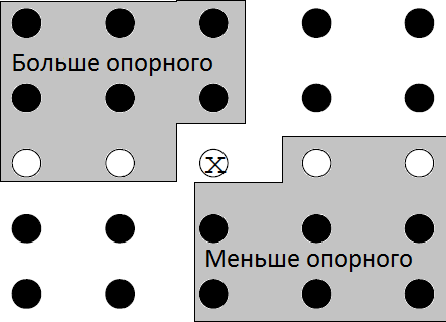
\includegraphics[width=0.7\linewidth]{img_easy/1_1.png}
	\captionsetup{labelformat=empty}
	\caption{Иллюстрация к рассуждению выше}
\end{figure}

Само время работы $T(n)$ не меньше, чем
\begin{enumerate}
	\item Время работы на сортировку группы (одна группа сортируется за константное время, так как в каждой группе константное количество элементов) и разбиение по рассекающему элементу (аналогично операции merge) --- $O(n)$
	\item времени работы для поиска медианы медиан, то есть $T\left(\frac{n}{5}\right)$
	\item времени работы для поиска $k$-го элемента в одной из двух частей массива, то есть $T(s)$, где s --- количество элементов в этой части. Но s
	не превосходит $\frac{7n}{10}$, так как чисел, меньших рассекающего элемента, не менее $\frac{3n}{10}$ --- это $\frac{n}{10}$
	медиан, меньших медианы медиан, плюс не менее 2n10
	элементов, меньших этих медиан. С другой стороны, чисел, больших рассекающего элемента, так же не менее $\frac{3n}{10}$, следовательно, $s \leq \frac{7n}{10}$, то есть в худшем случае $s=
	\frac{7n}{10}$.
\end{enumerate}

Итоговое время работы:
\[
	T(n) \leq T\left(\frac{7n}{10}\right) + T\left(\frac{n}{5}\right) + Cn
\]

Докажем по индукции, что $T(n) \leq 10Cn$

Предположим, что наше неравенство $T(n) \leq 10Cn$ выполняется при малых $n$, для некоторой достаточно большой константы $C$. 
Тогда, по предположению индукции, 

$$
T(n) \leq T\left(\frac{7n}{10}\right) + T\left(\frac{n}{5}\right) + Cn \leq 10C \cdot \frac{7n}{10} + 10C \cdot \frac{n}{5} + Cn = 10 Cn
$$
Значит, итоговая сложность алгоритма $O(n)$
\section{Сортировка массива: пузырьковая, mergesort, quicksort. Алгоритмы и оценки сложности.}


\textbf{Пузырьковая сортировка:}\\
Сложность: $O(n^2)$\\
Алгоритм: несколько раз проходимся по массиву, <<поднимая>> элемент в начало.

\textbf{Mergesort} (слияние)\\
Сложность: $T(n)=2T(\frac{n}{2})+O(n)$ или же $O(n\log n)$\\
Алгоритм: Разбиваем наш массив на 2, пока не останется по одному элементу, затем рекурсивно сравниваем каждый элемент с соседним, сортируем, объединяем.

\textbf{Quicksort}\\
Сложность в худшем случае --- $O(n^2)$, в среднем --- $O(n\log n)$\\
\textit{Алгоритм}:
\begin{enumerate}
	\item Выбрать из массива элемент, называемый опорным. Это может быть любой из элементов массива. От выбора опорного элемента не зависит корректность алгоритма, но может зависеть его эффективность.
	\item Сравнить все остальные элементы с опорным и переставить их в массиве так, чтобы разбить массив на три непрерывных отрезка, следующих друг за другом: <<элементы меньше опорного>>, <<равные>>, и <<большие>>.
	
	\item Для отрезков <<меньших>> и <<больших>> значений выполнить рекурсивно ту же последовательность операций, если длина отрезка больше единицы.
\end{enumerate}
\begin{figure}[!ht]
\centering
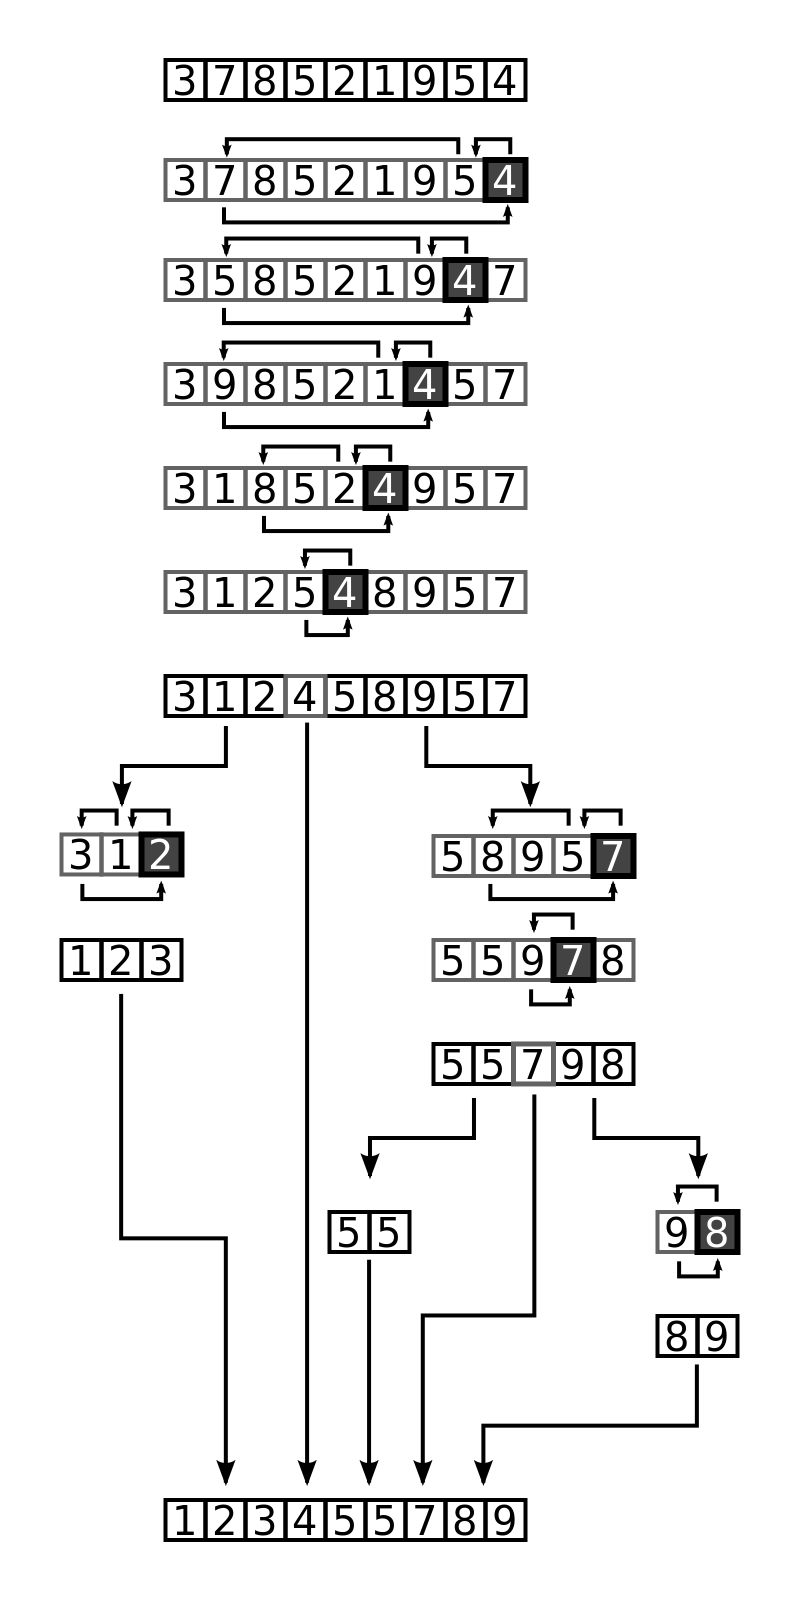
\includegraphics[width=0.2\textwidth]{img_easy/2_1.png}
\caption{\texttt{Quicksort}}
\end{figure}

\section{Списки: односвзяный и двусвязный}
\section{Бинарные деревья поиска. Вставка, удаление, оценки сложности.}



\section{Графы. Способы их представления в памяти компьютера. Матрицы смежости, матрицы инцедентности, списки связности, представление на двух массивах (CSR).}

На протяжении всего билета будем рассматривать граф на иллюстрации ниже

\begin{figure}[h!]
	\centering
	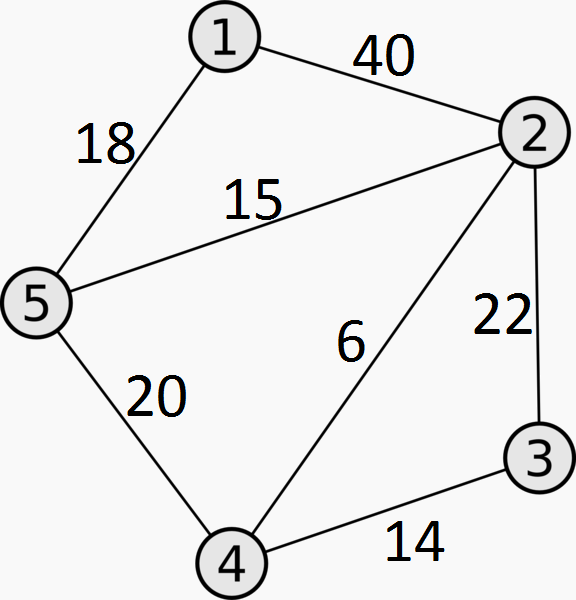
\includegraphics[width=0.4\linewidth]{img_easy/5_1.png}
	\captionsetup{labelformat=empty}
	\caption{}
	\label{fig:51}
\end{figure}

\subsection{Матрица смежности}

\begin{definition}
	Матрица смежности --- 
\end{definition}

\subsection{Матрица инцидентности}

\subsection{Списки смежности}

\subsection{CSR}
\section{Обходы графов. Обход в ширину, обход в глубину. }
\section{Алгоритмы поиска кратчайших путей. Алгоритм Дейкстры, алгоритм Беллмана-Форда. }
\section{Остовные деревья. Алгоритмы Прима, Краскала, Борувки.}
\section{Эвристики для поиска кратчайших путей, алгоритм A*.}
\section{Потоки в сетях. Максимальный поток и минимальный разрез.]}

См билет 6 из сложных
\section{ Хэш-функции. Коллизии. Хеш-таблицы.  Хэширование. Фильтр Блюма.}
\section{Предикат поворота. Задача пересечения двух отрезков}
\section{Выпуклые оболочки, алгоритма Джарвиса, Грэхема и QuickHull.}

\begin{definition}
	\textbf{Выпуклое множество} --- такое множество точек, что, для любых двух точек множества, все точки на отрезке между ними тоже принадлежат этому множеству.
\end{definition}

\begin{definition}
	\textbf{Выпуклая оболочка множества точек} --- такое выпуклое множество точек, что все точки фигуры также лежат в нем.
\end{definition}

\begin{definition}
	\textbf{Минимальная выпуклая оболочка множества точек} --- это минимальная по площади выпуклая оболочка.
\end{definition}

\subsection*{Алгоритмы построения выпуклой оболочки}

\subsection{Алгоритм Джарвиса}
По-другому "Gift wrapping algorithm" (Заворачивание подарка). Он заключается в том, что мы ищем выпуклую оболочку последовательно, против часовой стрелки, начиная с определенной точки.

\textbf{Описание алгоритма}

\begin{enumerate}
	\item Возьмем точку $p_0$ нашего множества с самой маленькой $у$ координатой (если таких несколько, берем самую правую из них). 
	Добавляем ее в ответ.
	\item На каждом следующем шаге для последнего добавленного pi
	ищем $p_i+1$ среди всех недобавленных точек и $p_0$
	с максимальным полярным углом относительно $p_i$ (Если углы равны, надо сравнивать по расстоянию). Добавляем pi+1 в ответ. 
	Если $p_i+1==p_0$, заканчиваем алгоритм
\end{enumerate}

\begin{figure}[h!]
	\centering
	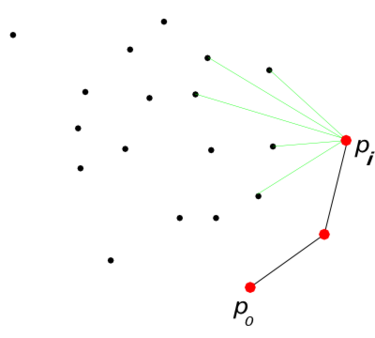
\includegraphics[width=0.4\linewidth]{img_easy/13_1.png}
	\captionsetup{labelformat=empty}
	\caption{Промежуточный шаг алгоритма. 
		Для точки $p_i$ ищем следующую перебором.}
\end{figure}
\textbf{Корректность}
Точка $p_0$, очевидно, принадлежит оболочке. На каждом последующем шаге алгоритма мы получаем прямую $p_{i-1}pi$, по построению которой все точки множества лежат слева от нее. 
Значит, выпуклая оболочка состоит из $p_i$-х и только из них.

\textbf{Сложность}

Добавление каждой точки в ответ занимает $O(n)$ времени, всего точек будет $k$, поэтому итоговая сложность $O(nk)$. В худшем случае, когда оболочка состоит из всех точек сложность $O(n^2)$.

\subsection{Алгоритм Грэхема}
Алгоритм заключается в том, что мы ищем точки оболочки последовательно, используя стек.

\textbf{Описание алгоритма}

\begin{enumerate}
	\item Находим точку $p_0$
	нашего множества с самой маленькой у-координатой (если таких несколько, берем самую правую из них), добавляем в ответ.
	\item Сортируем все остальные точки по полярному углу относительно $p_0$.
	\item Добавляем в ответ $p_1$ --- самую первую из отсортированных точек.
	\item Берем следующую по счету точку t.
	Пока t и две последних точки в текущей оболочке $p_i$ и $p_i-1$ образуют неправый поворот (вектора $p_it$ и $p_{i-1}p_i$), удаляем из оболочки $p_i$.
	\item Добавляем в оболочку $t$.
	\item Делаем п.4, пока не закончатся точки
\end{enumerate}

\subsection*{Корректность}

Докажем, что на каждом шаге множество $P_i$-тых является выпуклой оболочкой всех уже рассмотренных точек. Доказательство проведем по индукции.

\begin{itemize}
	\item \textbf{База.} Для трёх первых точек утверждение, очевидно, выполняется.
	\item \textbf{Переход.} Пусть для $i-1$ точек оболочки совпадают. Докажем, что и для $i$ точек они совпадут.
\end{itemize}

Рассмотрим истинную оболочку $ch(S \cup i) = ch(S) \cup i \setminus P$, где $P$ --- множество всех точек из $ch(S)$, видимых из $i$. Так как мы добавляли точки в нашу оболочку против часовой стрелки и так как $i$-тая точка лежит в $ch(S \cup i)$, то $P$ состоит из нескольких подряд идущих последних добавленных в оболочку точек, и именно их мы удаляем на текущем шаге. Поэтому наша оболочка и истинная для $i$ точек совпадают.

Тогда по индукции оболочки совпадают и для $i = n$.

\subsection*{Сложность}

Сортировка точек занимает $O(n \log n)$ времени. При обходе каждая точка добавляется в ответ не более одного раза, поэтому сложность этой части --- $O(n)$. Суммарное время --- $O(n \log n)$.

\subsection{Алгоритм QuickHull}

Попытаемся применить к этой задаче подход <<Разделяй и властвуй>>

\subsection*{Описание Алгоритма}

\begin{enumerate}
	\item Найдем самую левую точку $p_0$ и самую правую точку $p_1$ (Если таких несколько, выберем среди таких нижнюю и верхнюю соответственно).
	\item Возьмем все точки выше прямой $p_0 p_1$.
	\item Найдем среди этого множества точку $p_i$, наиболее отдаленную от прямой (если таких несколько, взять самую правую).
	\item Рекурсивно повторить шаги 2-3 для прямых $p_0 p_i$ и $p_i p_1$, пока есть точки.
	\item Добавить в ответ точки $p_0 \dots p_i \dots p_1$, полученные в п. 3.
	\item Повторить пункты 2-5 для $p_1 p_0$ (то есть для "нижней" половины).
	\item Ответ - объединение списков из п. 5 для верхней и нижней половины.
\end{enumerate}

\subsection*{Сложность}

Пусть время, необходимое для нахождения оболочки над некой прямой и множеством точек $S$ есть $T(S)$. Тогда
$T(S) = O(\|S\|) + T(A \in S) + T(B \in S)$, где $A, B$ --- множества над полученными прямыми. Отсюда видно, что в худшем случае, алгоритм тратит $O(n^2)$. На случайных же данных это число равно $O(n \log n)$.

\section{kD-деревья. Окто- и квадро-деревья.}
\section{Многочлены. Метод Горнера. Умножение Карацубы.}


\setcounter{section}{0} 
\section{Основная теорема для рекуррентных соотношений. Схема доказательства.}

\textbf{Теорема\\}
 Пусть $T(n)=a\cdot T(\lceil n/b\rceil)+O(n^d)$. Тогда
$$
T(n)=\begin{cases}O(n^d), &d>\log_ba\\O(n^d\log n), &d=\log_ba\\O(n^{\log_ba}), &d<\log_ba\end{cases},
$$

где $a \ge 1$ --- количество частей, на которые мы дробим задачу, $b>1$ --- во сколько раз легче становится решить задачу, $d$ --- степень сложности входных данных.
%\begin{comment}
%	Здесь подразумевается, что $T(1)=O(1)$.\\
%	Пример дерева рекурсий вы видели ранее в 7 билете.
%\end{comment} 



\textbf{Схема доказательства:}\\
Рассмотрим дерево рекурсии данного соотношения. Всего в нем будет $\log_bn$ уровней. На каждом таком уровне, количество детей в дереве будет умножаться на $a$ $\>$~на уровне $i$ будет $a^i$ потомков. Также известно, что каждый ребенок на уровне $i$ размера $\dfrac{n}{b^i}$. Ребенок размера $\dfrac{n}{b^i}$ требует $O\bigg(\Big(\dfrac{n}{b^i}\Big)^d\bigg)$ дополнительных затрат, поэтому общее количество совершенных действий на уровне $i$: $$O\left(a^i\cdot\left(\frac{n}{b^i}\right)^d\right)=O\left(n^d\cdot\Big(\frac{a^i}{b^{id}}\Big)\right)=O\left(n^d\cdot\left(\frac{a}{b^d}\right)^i\right)$$
Решение разбивается на три случая: когда $\dfrac{a}{b^d}$ больше 1, равна 1 или меньше 1. Переход между этими случаями осуществляется при
$$\frac{a}{b^d}=1\Leftrightarrow a=b^d\Leftrightarrow\log_ba=d\cdot\log_bb\Leftrightarrow\log_ba=d$$
Распишем всю работу в течение рекурсивного спуска:
$$T(n)=\sum\limits_{i=0}^{\log_bn}O\left(n^d\left(\frac{a}{b^d}\right)^i\right)+O(1)=O\Bigg(n^d\cdot\sum\limits_{i=0}^{\log_bn}\left(\frac{a}{b^d}\right)^i\Bigg)$$
Отсюда получаем:
\begin{enumerate}
	\item $d>\log_ba\Rightarrow T(n)=O(n^d)$ (так как $\left(\dfrac{a}{b^d}\right)^i$ --- бесконечно убывающая геометрическая прогрессия)
	\item $d=\log_ba\Rightarrow T(n)=O\Bigg(n^d\cdot\sum\limits_{i=0}^{\log_bn}\left(\dfrac{a}{b^d}\right)^i\Bigg)=$\\
	$=O\Bigg(n^d\cdot\sum\limits_{i=0}^{\log_bn}\left(1\right)^i\Bigg)=O(n^d+n^d\cdot\log_bn)=O(n^d\cdot\log_bn)$
	\item $d<\log_ba\Rightarrow T(n)=O\Bigg(n^d\cdot\sum\limits_{i=0}^{\log_bn}\left(\dfrac{a}{b^d}\right)^i\Bigg)=O\left(n^d\cdot\left(\dfrac{a}{b^d}\right)^{\log_bn}\right)$, но $$n^d\cdot\left(\frac{a}{b^d}\right)^{\log_bn}=n^d\cdot\left(\frac{a^{\log_bn}}{b^{d\log_bn}}\right)=n^d\cdot\left(\frac{n^{\log_ba}}{n^d}\right)=n^{\log_ba}\Rightarrow T(n)=O(n^{\log_ba})$$
\end{enumerate}
\section{АВЛ-деревья. Повороты, балансировка.}


АВЛ-дерево - сбалансированное двоичное дерево поиска со следующим свойством: для каждой его вершины высота её двух поддеревьев различается не более чем на 1.
Названо в честь изобретателей  Г. М. Адельсона-Вельского и Е. М. Ландиса.

\textbf{Теорема:} АВЛ-дерево имеет высоту $h=O(\log n)$.

\textbf{Доказательство:} Высоту поддерева с корнем $x$ будем обозначать как $h(x)$.
Пусть $m_h$ - минимальное число вершин в АВЛ-дереве высоты $h$. Тогда легко видеть, что $m_{h+2}=m_{h+1}+m_h+1$ по индукции.
Равенством $m_h=F_{h+2}-1$ докажем.

\textbf{База:} $m_1=F_3-1$ - верно, $m_1=1$, $F_3=2$.

\textbf{Шаг:} Допустим $m_h=F_{h+2}-1$ - верно.
Тогда $m_{h+1}=m_h+m_{h-1}+1=F_{h+2}-1+F_{h+1}-1+1 = F_{h+3}-1$.

$F_h=\Omega(\varphi^h)$ где $\varphi=\frac{\sqrt{5}+1}{2}$.
То есть $n \ge \varphi^h \Rightarrow \log_{\varphi} n \ge h$.
Высота АВЛ-дерева из $n$ вершин - $O(\log n)$.

\textbf{Балансировка:}
Балансировкой вершины называется операция, которая в случае разницы высот левого и правого поддеревьев $|h(L)-h(R)|=2$ изменяет связи предок - потомок в поддереве данной вершины так, чтобы восстановилось свойство дерева $|h(L)-h(R)|=1$, иначе ничего не меняет.
$(diff[i]=h(L)-h(R))$.

\textbf{Малое вращение: ($O(1)$)}
\begin{itemize}
	\item Левое используется когда $h(b)-h(L)=2$ и $h(c) \le h(R)$.
	\item Правое используется, когда $h(a)-h(R)=2$ и $h(c) \le h(L)$.
\end{itemize}



\textbf{Большое вращение: ($O(1)$)}
Левое используется когда $h(b)-h(L)=2$ и $h(c)>h(R)$.
Правое используется когда $h(b)-h(R)=2$ и $h(c)>h(L)$.


Большое вращение состоит из двух малых.

\textbf{Вставка (insert):}
Спускаемся по дереву, как при поиске.
Если мы стоим в вершине $a$ и там надо идти в поддерево $b$, то делаем $b$ листом, а вершину $a$ корнем.
Поднимаемся вверх по пути поиска и пересчитываем баланс у вершин.
Если мы поднялись в вершину $i$ из левого поддерева, то $diff[i]=h(L)-h(R)$ увеличилось на 1. Если из правого - уменьшается на 1.
Если пришли в вершину и баланс стал равен 0, то высота не изменилась и подъём останавливается.
Если пришли в вершину и её баланс стал равен 1 или -1, то высота поддерева изменилась и подъём продолжается.
Если пришли в вершину и её баланс стал равен 2 или -2, то делаем одно из 4 вращений и, если после вращения баланс стал 0, то останавливаемся, иначе продолжаем подъём.
Сложность: $O(\log n)$, т.к. в процессе добавления вершины мы рассматриваем не более $O(\log n)$ вершин, и для каждой запускаем балансировку не более одного раза.

\textbf{Удаление (delete):}
Если вершина лист, удаляем её.
Иначе найдём самую близкую по значению вершину и, переместим её на место удаляемой вершины, а затем удалим эту вершину.
От удалённой вершины будем подниматься к корню и пересчитывать баланс у вершин.
$diff[]$ уменьшается.
Если поднялись из левого поддерева, то $diff[]$ уменьшается на 1. Если из правого - увеличивается на 1.
Если пришли в вершину и её баланс стал равен 1 или -1, то высота поддерева не изменилась и подъём можно остановить.
Если пришли в вершину и баланс стал равен 0, то высота поддерева уменьшилась и подъём нужно продолжить.
Если пришли в вершину и её баланс стал равен 2 или -2, то делаем одно из 4 вращений и, если после вращения баланс стал 0, то подъём продолжается, иначе - останавливается.
Аналогично с вставкой: $O(\log n)$.

\textbf{Поиск (find):}
Как в обычном бинарном дереве поиска. $O(\log n)$.
\section{Красно-черные деревья. Балансировка (схема).}
\section{Бинарные кучи. Реализация с указателями и на массиве. Добавление и удаление элемента в бинарную кучу. }

\begin{definition}
    Двоичная куча или пирамида (англ. Binary heap) --- такое двоичное дерево, для которого выполнены следующие три условия:

    \begin{enumerate}
        \item Значение в любой вершине не больше (если куча для минимума), чем значения в её потомках.
        \item На $i$-м слое (кроме, может быть, последнего) $2^i$ вершин. Слои нумеруются с нуля.
        \item Последний слой заполнен слева направо.
    \end{enumerate}
\end{definition}

Удобнее всего двоичную кучу хранить в виде массива $a[0..n-1]$, у которого нулевой элемент, $a[0]$ --- элемент в корне, а потомками элемента $a[i]$ являются $a[2i+1]$ и $a[2i+2]$.
Высота кучи определяется как высота двоичного дерева.
То есть она равна количеству рёбер в самом длинном простом пути, соединяющем корень кучи с одним из её листьев.
Высота кучи есть $O(\log n)$, где $n$ --- количество узлов дерева.

Чаще всего используют кучи для минимума (когда предок не больше детей) и для максимума (когда предок не меньше детей).

Двоичные кучи используют, например, для того, чтобы извлекать минимум из набора чисел за $O(\log n)$.
Они являются частным случаем приоритетных очередей.

\subsection{Восстановление свойств кучи}

Если в куче изменяется один из элементов, то она может перестать удовлетворять свойству упорядоченности.
Для восстановления этого свойства служат процедуры siftDown (просеивание вниз) и siftUp (просеивание вверх). 

\subsubsection{siftDown}

Если значение измененного элемента увеличивается, то свойства кучи восстанавливаются функцией siftDown.

Работа процедуры: если $i$-й элемент меньше, чем его сыновья, всё поддерево уже является кучей, и делать ничего не надо.
В противном случае меняем местами $i$-й элемент с наименьшим из его сыновей, после чего выполняем siftDown для этого сына.
Процедура выполняется за время $O(\log n)$.

\begin{verbatim}
function siftDown(i : int):
    while 2 * i + 1 < a.heapSize     // heapSize — количество элементов в куче
        left = 2 * i + 1             // left — левый сын
        right = 2 * i + 2            // right — правый сын
        j = left
        if right < a.heapSize and a[right] < a[left]
            j = right
        if a[i] <= a[j]
            break
        swap(a[i], a[j])
        i = j
\end{verbatim}

\subsubsection{siftUp}

Если значение измененного элемента уменьшается, то свойства кучи восстанавливаются функцией siftUp.

Работа процедуры: если элемент больше своего отца, условие 1 соблюдено для всего дерева, и больше ничего делать не нужно.
В противном случае мы меняем местами его с отцом, после чего выполняем siftUp для этого отца.
Иными словами, слишком маленький элемент всплывает наверх.
Процедура выполняется за время $O(\log n)$.

\begin{verbatim}
function siftUp(i : int):
    while a[i] < a[(i - 1) / 2]     // i  0 — мы в корне
        swap(a[i], a[(i - 1) / 2])
        i = (i - 1) / 2
\end{verbatim}

\subsection{Извлечение минимального элемента}

Выполняет извлечение минимального элемента из кучи за время $O(\log n)$.
Извлечение выполняется в четыре этапа:

\begin{enumerate}
    \item Значение корневого элемента (он и является минимальным) сохраняется для последующего возврата.
    \item Последний элемент копируется в корень, после чего удаляется из кучи.
    \item Вызывается siftDown для корня.
    \item Сохранённый элемент возвращается.
\end{enumerate}

\begin{verbatim}
int extractMin():
    int min = a[0]
    a[0] = a[a.heapSize - 1]
    a.heapSize = a.heapSize - 1
    siftDown(0)
    return min
\end{verbatim}

\subsection{Добавление нового элемента}

Выполняет добавление элемента в кучу за время $O(\log n)$.
Сначала производится добавление произвольного элемента в конец кучи, затем восстановление свойства упорядоченности с помощью процедуры siftUp.

\begin{verbatim}
function insert(key : int):
    a.heapSize = a.heapSize + 1
    a[a.heapSize - 1] = key
    siftUp(a.heapSize - 1)
\end{verbatim}

\section{Очереди с приоритетами. Наивная реализация, реализация на бинарной куче. }
\section{Потоки в сетях. Задача о максимальном потоке. Алгоритм Форда – Фалкерсона. }
\section{Амортизационный анализ: групповой анализ, банковский метод. Амортизационный анализ для бинарного счётчика }

\textbf{Амортизационный анализ:}
Метод анализа производительности алгоритмов, учитывающий общую стоимость последовательности операций, а не только стоимость одной.
Идея:
\begin{itemize}
	\item Пересчитать на более скрытые или редкие операции.
	\item Стоимость операции как бы <<размазывается>> на все операции, входящие в последовательность.
	\item Отражает наихудший случай.
	\item Не учитывает вероятность.
\end{itemize}

\textbf{Метод группировки:}
В случае, когда в наихудшем случае суммарное время выполнения $k$ операций $T_k(N)$ не зависит от $N$, то амортизированная стоимость каждой операции $A(N) = T_k(N)/k$.

\subsection*{Пример: Бинарный счетчик}
Счетчик имеет $n$ бит (например, $N$ значений).
Поддерживает операции $Increment$ и $Reset$.
Пусть $N=5$. Изначально счетчик равен 00000.
Пример:\\
0. 00000\\
1. 00001\\
2. 00010\\
3. 00011\\
4. 00100\\

За $N$ элементов каждый раз $k$ операций. $k$ - количество операций.
Например, для $N=4$:
000 $\rightarrow$ 001 (1 раз)
001 $\rightarrow$ 010 (2 раза)
010 $\rightarrow$ 011 (1 раз)
011 $\rightarrow$ 100 (3 раза)
$\Rightarrow$ $N$ бит менялись $k$ раз.

Тогда амортизированная стоимость $O(k)$, где $k=2N$.
$A(N) = N + \frac{N}{2} + \frac{N}{4} + \dots + 1 = 2N$.
Сложность $O(1)$.

\subsection*{Бухгалтерский метод (взвешивания)}
1. На операции тратится столько условных единиц, сколько больше (меньше) реально.

2. Если уж стоит и реально получится, то разность сил и цен на $k$-ю операцию.

3. Условные деньги вводится так, чтобы их хватало на любые операции. Это для того, чтобы кредит не были отрицательными деньги.

\section{Амортизационный анализ: метод потенциалов для динамического массива. }
\section{Алгоритм Рабина --- Карпа, алгоритм Кнута --- Морриса -- Пратта.  Структура данных «бор», алгоритм Ахо --- Корасик}

\subsection{Алгоритм Рабина --- Карпа}

Алгоритм Рабина --- Карпа предназначен для поиска подстроки в строке.
Наивный алгоритм поиска подстроки в строке работает за $O(n^2)$ в худшем случае --- слишком долго.
Чтобы ускорить этот процесс, можно воспользоваться методом хеширования.

\begin{definition}
    Пусть дана строка $s[0..n-1]$. Тогда \textbf{полиномиальным хешем} (англ. polynomial hash) строки $s$ называется число $h=hash(s[0..n-1])=p^0 s[0]+...+p^{n-1}s[n-1]$, где $p$ --- некоторое простое число, а $s[i]$ --- код $i$-го символа строки s.
\end{definition}

Проблему переполнения при вычислении хешей довольно больших строк можно решить так --- считать хеши по модулю $r=2^{64}$ (или $2^{32}$), чтобы модуль брался автоматически при переполнении типов.
Для работы алгоритма потребуется считать хеш подстроки $s[i..j]$.
Делать это можно следующим образом:

Рассмотрим хеш s[0..j]: $$hash(s[0..j])=s[0]+ps[1]+...+p^{i-1}s[i-1]+p^is[i]+...+p^{j-1}s[j-1]+p^js[j].$$
Разобьем это выражение на две части: $$hash(s[0..j])=(s[0]+ps[1]+...+p^{i-1}s[i-1])+(p^is[i]+...+p^{j-1}s[j-1]+p^js[j]).$$
Вынесем из последней скобки множитель $p^i$: $$hash(s[0..j])=(s[0]+ps[1]+...+p^{i-1}s[i-1])+p^i(s[i]+...+p^{j-i-1}s[j-1]+p^{j-i}s[j]).$$
Выражение в первой скобке есть не что иное, как хеш подстроки $s[0..i-1]$, а во второй --- хеш нужной нам подстроки $s[i..j]$.
Итак, мы получили, что: $$hash(s[0..j])=hash(s[0..i-1])+p^ihash(s[i..j]).$$
Отсюда получается следующая формула для $hash(s[i..j])$: $$hash(s[i..j])=(1/p^i)(hash(s[0..j])-hash(s[0..i-1])).$$

Однако, как видно из формулы, чтобы уметь считать хеш для всех подстрок, начинающихся с $i$, нужно предпосчитать все $p^i$ для $i \in [0..n-1]$.
Это займет много памяти.
Но поскольку нам нужны только подстроки размером $m$, мы можем подсчитать хеш подстроки $s[0..m-1]$, а затем пересчитывать хеши для всех $i \in [0..n-m]$ за $O(1)$ следующим образом: $$hash(s[i+1..i+m-1])=(hash(s[i..i+m-1])-p^{m-1}s[i])\mod r.$$
$$hash(s[i+1..i+m])=(p \cdot hash(s[i+1..i+m-1])+s[i+m])\mod r.$$
Получается: $$hash(s[i+1..i+m])=(p \cdot hash(s[i..i+m-1])-p^is[i]+s[i+m]) \mod r.$$

\subsubsection{Алгоритм}

Алгоритм начинается с подсчета $hash(s[0..m-1])$ и $hash(p[0..m-1])$, а также с подсчета $p^m$, для ускорения ответов на запрос.

Для $i \in [0..n-m]$ вычисляется $hash(s[i..i+m-1])$ и сравнивается с $hash(p[0..m-1])$.
Если они оказались равны, то образец $p$, скорее всего, содержится в строке $s$ начиная с позиции $i$, хотя возможны и ложные срабатывания алгоритма.
Если требуется свести такие срабатывания к минимуму или исключить вовсе, то применяют сравнение некоторых символов из этих строк, которые выбраны случайным образом, или применяют явное сравнение строк, как в наивном алгоритме поиска подстроки в строке.
В первом случае проверка произойдет быстрее, но вероятность ложного срабатывания, хоть и небольшая, останется.
Во втором случае проверка займет время, равное длине образца, но полностью исключит возможность ложного срабатывания.

Если требуется найти индексы вхождения нескольких образцов, или сравнить две строки --- выгоднее будет предпосчитать все степени $p$, а также хеши всех префиксов строки $s$.

\subsubsection{Псевдокод}

Приведем пример псевдокода, который находит все вхождения строки $w$ в строку $s$ и возвращает массив позиций, откуда начинаются вхождения.

\begin{minted}{c++}
vector<int> rabinKarp (s : string, w : string):
   vector<int> answer
   int n = s.length
   int m = w.length
   int hashS = hash(s[0..m - 1])
   int hashW = hash(w[0..m - 1])
   for i = 0 to n - m
        if hashS == hashW
             answer.add(i)
        hashS = (p * hashS - pm

 * hash(s[i]) + hash(s[i + m])) mod r // r — некоторое большое число, p — некоторое просто число
   return answer
\end{minted}

Новый хеш $hashS$ был получен с помощью быстрого пересчёта.
Для сохранения корректности алгоритма нужно считать, что $s[n+1]$ --- пустой символ.

\subsubsection{Время работы}

Изначальный подсчёт хешей выполняется за $O(m)$.
Каждая итерация выполняется за $O(1)$.
В цикле всего $n-m+1$ итераций.
Итоговое время работы алгоритма $O(n+m)$.

Однако если требуется исключить ложные срабатывания алгоритма полностью, т.е. придется проверить все полученные позиции вхождения на истинность, то в худшем случае итоговое время работы алгоритма будет $O(n \cdot m)$.

\subsection{Алгоритм Кнута --- Морриса --- Пратта}

Алгоритм Кнута --- Морриса --- Пратта (англ. Knuth–Morris–Pratt algorithm) --- алгоритм поиска подстроки в строке.

\subsubsection{Алгоритм}

Дана цепочка $T$ и образец $P$.
Требуется найти все позиции, начиная с которых $P$ входит в $T$.
Построим строку $S=P\#T$, где $\#$ --- любой символ, не входящий в алфавит $P$ и $T$.
Посчитаем на ней значение префикс-функции $p$.
Благодаря разделительному символу $\#$ выполняется $\forall i:p[i] \le |P|$.
Заметим, что по определению префикс-функции при $i>|P|$ и $p[i]=|P|$ подстроки длины $P$, начинающиеся с позиций 0 и $i-|P|+1$, совпадают.
Соберем все такие позиции $i-|P|+1$ строки $S$, вычтем из каждой позиции $|P|+1$, это и будет ответ.
Другими словами, если в какой-то позиции $i$ выполняется условие $p[i]=|P|$, то в этой позиции начинается очередное вхождение образца в цепочку.

\subsubsection{Псевдокод}

\begin{minted}{c}
int[] kmp(string P, string T):
   int pl = P.length
   int tl = T.length
   int[] answer
   int[] p = prefixFunction(P + "#" + T)
   int count = 0
   for i = 0 .. tl - 1
      if p[pl + i + 1] == pl
         answer[count++] = i - pl
   return answer
\end{minted}

\subsubsection{Время работы}

Префикс-функция от строки $S$ строится за $O(S)=O(P+T)$.
Проход цикла по строке $S$ содержит $O(T)$ итераций.
Суммарное время работы алгоритма оценивается как $O(P+T)$. 

\subsubsection{Оценка по памяти}

Предложенная реализация имеет оценку по памяти $O(P+T)$.
Оценки $O(P)$ можно добиться за счет запоминания значений префикс-функции для позиций в $S$, меньших $|P|+1$ (то есть до начала цепочки $T$).
Это возможно, так как значение префикс-функции не может превысить длину образца благодаря разделительному символу $\#$. 

\subsection{Структура данных «бор»}

\begin{definition}
    \textbf{Бор} (англ. trie, луч, нагруженное дерево) --- структура данных для хранения набора строк, представляющая из себя дерево с символами на рёбрах.
    Строки получаются последовательной записью всех символов, хранящихся на рёбрах между корнем бора и терминальной вершиной.
    Размер бора линейно зависит от суммы длин всех строк, а поиск в бору занимает время, пропорциональное длине образца. 
\end{definition}

\subsubsection{Пример}

Бор для набора образцов \{he, she, his, hers\}:

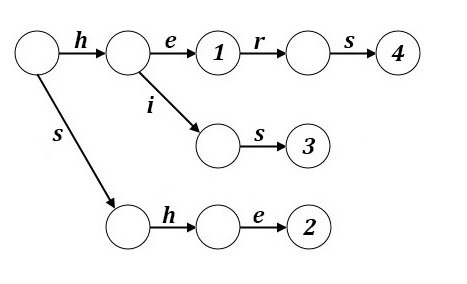
\includegraphics[]{img/9_1.jpg}

\subsubsection{Построение}

Введем следующие обозначения:

\begin{enumerate}
    \item $S$ --- используемый алфавит;
    \item $P={P_1,…,P_k}$ --- набор строк над $S$, называемый словарём;
    \item $n = \sum_{i = 1}^k |P_i|$ --- сумма длин строк.
\end{enumerate}

Бор храним как набор вершин, у каждой из которых есть метка, обозначающая, является ли вершина терминальной и указатели (рёбра) на другие вершины или на NULL.

\begin{minted}{c}
struct vertex:
    vertex next[|S|] 
    bool isTerminal
\end{minted}

\begin{enumerate}
    \item Создадим дерево из одной вершины (в нашем случае --- корня).
    \item Добавление элементов в дерево.
    Добавляем шаблоны $P_i$ один за другим.
    Следуем из корня по рёбрам, отмеченным буквами из $P_i$, пока возможно.
    Если $P_i$ заканчивается в $v$, сохраняем идентификатор $P_i$ (например, $i$) в $v$ и отмечаем вершину $v$ как терминальную.
    Если ребра, отмеченного очередной буквой $P_i$, нет, то создаем новое ребро и вершину для символа строки $P_i$.
\end{enumerate}

Построение занимает, очевидно, $O(|P_1|+...+|P_k|)=O(n)$ времени, так как поиск буквы, по которой нужно переходить, происходит за $O(1)$.
Поскольку на каждую вершину приходится $O(|S|)$ памяти, то использование памяти есть $O(n|S|)$. 

\subsection{Алгоритм Ахо --- Корасик.}

Пусть дан набор строк в алфавите размера $k$ суммарной длины $m$.
Необходимо найти для каждой строки все ее вхождения в текст.

\subsubsection{Шаг 1. Построение бора}

Строим бор из строк.
Построение выполняется за время $O(m)$, где $m$ --- суммарная длина строк.

\subsubsection{Шаг 2. Преобразование бора}

Обозначим за $[u]$ слово, приводящее в вершину $u$ в боре.
Узлы бора можно понимать как состояния автомата, а корень как начальное состояние.
Узлы бора, в которых заканчиваются строки, становятся терминальными.
Для переходов по автомату заведём в узлах несколько функций:

\begin{enumerate}
    \item $parent(u)$ — возвращает родителя вершины u;
    \item $\pi(u)=\delta(\pi(parent(u)),c)$ --- \textbf{суффиксная ссылка}, и существует переход из $parent(u)$ в $u$ по символу $c$;
    \item Функция перехода $\delta(u, c)=\begin{cases}
    v, \text{если из $u$ в $v$ ведёт символ $c$};\\
    root, \text{если $u$ --- корень и из него не исходит символ $c$};\\
    \delta(\pi(u), c), \text{иначе}.
    \end{cases}$
\end{enumerate}

Мы можем понимать рёбра бора как переходы в автомате по соответствующей букве.
Однако одними только рёбрами бора нельзя ограничиваться.
Если мы пытаемся выполнить переход по какой-либо букве, а соответствующего ребра в боре нет, то мы тем не менее должны перейти в какое-то состояние.
Для этого нам и нужны суффиксные ссылки.
Суффиксная ссылка $\pi(u)=v$, если $[v]$ --- максимальный суффикс $[u]$, $[v]\not=[u]$.
Функции перехода и суффиксные ссылки можно найти либо алгоритмом обхода в глубину с ленивыми вычислениями, либо с помощью алгоритма обхода в ширину. 

Из определений выше можно заметить два следующих факта:

\begin{itemize}
    \item функция перехода определена через суффиксную ссылку, а суффиксная ссылка — через функию переходов;
    \item для построения суффиксных ссылок небходимо знать информацию только выше по бору от текущей вершины до корня.
\end{itemize}

Это позволяет реализовать функции поиска переходов по символу и суффиксных ссылок ленивым образом при помощи взаимной рекурсии.

\subsubsection{Пример автомата Ахо-Корасик}

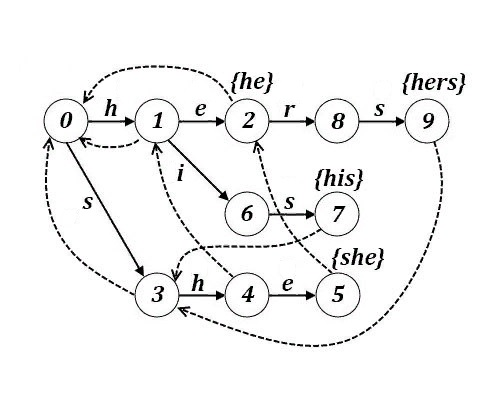
\includegraphics[]{img/9_2.jpg}

Пунктиром обозначены суффиксные ссылки.
Из вершин, для которых они не показаны, суффиксные ссылки идут в корень.

Суффиксная ссылка для каждой вершины $u$ --- это вершина, в которой оканчивается наидлиннейший собственный суффикс строки, соответствующей вершине $u$.
Единственный особый случай --- корень бора: для удобства суффиксную ссылку из него проведём в себя же.
Например, для вершины 5 с соответствующей ей строкой \textbf{she} максимальным подходящим суффиксом является строка \textbf{he}.
Видим, что такая строка заканчивается в вершине 2.
Следовательно суффиксной ссылкой вершины для 5 является вершина 2. 

\subsubsection{Шаг 3. Построение сжатых суффиксных ссылок}

При построении автомата может возникнуть такая ситуация, что ветвление есть не на каждом символе.
Тогда можно маленький бамбук заменить одним ребром.
Для этого и используются сжатые суффиксные ссылки.

$$up(u) = \begin{cases}
    \pi(u), \text{если $\pi(u)$ --- терминальная};\\
    \emptyset, \text{если $\pi(u)$ --- корень};\\
    up(\pi(u)), \text{иначе}.
\end{cases}$$

Здесь $up$ --- сжатая суффиксная ссылка, т.е. ближайшее допускающее состояние (терминал) перехода по суффиксным ссылкам.
Аналогично обычным суффиксным ссылкам, сжатые суффиксные ссылки могут быть найдены при помощи ленивой рекурсии.

\subsubsection{Использование автомата}

По очереди просматриваем символы текста.
Для очередного символа $c$ переходим из текущего состояния $u$ в состояние, которое вернёт функция $\delta(u,c)$.
Оказавшись в новом состоянии, отмечаем по сжатым суффиксным ссылкам строки, которые нам встретились, и их позицию (если требуется).
Если новое состояние является терминальным, то соответствующие ему строки тоже отмечаем.

\section{Алгоритм Бойера-Мура. Эвристики стоп-символа и хорошего суффикса. [7]}
\section{Расстояние Левенштейна, алгоритм Вагнера --- Фишера}

\begin{definition}
    Расстояние Левенштейна (англ. Levenshtein distance) (также редакционное расстояние или дистанция редактирования) между двумя строками в теории информации и компьютерной лингвистике --- это минимальное количество операций вставки одного символа, удаления одного символа и замены одного символа на другой, необходимых для превращения одной строки в другую.
\end{definition}

Для расстояния Левенштейна справедливы следующие утверждения:

\begin{itemize}
    \item $d(S_1,S_2) \ge \big||S_1|-|S_2| \big|,$
    \item $d(S_1,S_2) \le \max(|S_1|,|S_2|),$
    \item $d(S_1,S_2)=0 \Leftrightarrow S_1=S_2,$
\end{itemize}

где $d(S_1,S_2)$ --- расстояние Левенштейна между строками $S_1$ и $S_2$, а $|S|$ --- длина строки $S$.
Расстояние Левенштейна является метрикой. Для того, чтобы доказать это, достаточно доказать, что выполняется неравенство треугольника:
\begin{itemize}
    \item $d(S_1,S_3) \le d(S_1,S_2) + d(S_2,S_3).$
\end{itemize}

Пусть $d(S_1,S_3) = x$, $d(S_1,S_2) = y$, $d(S_2,S_3) = z$.
Тогда $x$ --- кратчайшее редакционное расстояние от $S_1$ до $S_3$, $y$ --- кратчайшее редакционное расстояние от $S_1$ до $S_2$, а $z$ --- кратчайшее редакционное расстояние от $S_2$ до $S_3$.
При этом $y+z$ --- какое-то расстояние от $S_1$ до $S_3$.
В других случаях $d(S_1,S_3) < d(S_1,S_2) + d(S_2,S_3).$
Следовательно, выполняется неравенство треугольника.

Рассмотрим более общий случай: пусть цены операций могут зависеть от вида операции (вставка, удаление, замена) и/или от участвующих в ней символов.

\begin{lemma}
    Будем считать, что элементы строк нумеруются с первого, как принято в математике, а не нулевого.
    Пусть $S_1$ и $S_2$ --- две строки (длиной $M$ и $N$ соответственно) над некоторым алфавитом, тогда редакционное расстояние $d(S_1,S_2)$ можно подсчитать по следующей рекуррентной формуле: $d(S_1,S_2) = D(M, N)$, где
    \begin{equation*}
        D(i, j) = 
        \begin{cases}
            0 &;i = 0, j = 0\\
            i \cdot deleteCost &;j = 0, i > 0\\
            j \cdot insertCost &;i = 0, j > 0\\
            D(i-1,j-1) &;S_1[i] = S_2[j]\\
            \min(D(i, j - 1) + insertCost,\\
            \ \ \ \ \ \ \ \ D(i - 1, j) + deleteCost, &;i > 0, j > 0, S_1[i] \not= S_2[j]\\
            \ \ \ \ \ \ \ \ D(i - 1, j - 1) + replaceCost).
        \end{cases}
    \end{equation*}
\end{lemma}
\begin{proof}
    Рассмотрим формулу более подробно.
    Здесь $D(i,j)$ --- расстояние между префиксами строк: первыми $i$ символами строки $S_1$ и первыми $j$ символами строки $S_2$.
    Очевидно, что редакционное расстояние между двумя пустыми строками равно нулю.
    Также очевидно то, что чтобы получить пустую строку из строки длиной $i$, нужно совершить $i$ операций удаления, а чтобы получить строку длиной $j$ из пустой, нужно произвести $j$ операций вставки.
    Осталось рассмотреть нетривиальный случай, когда обе строки непусты.

    Для начала заметим, что в оптимальной последовательности операций их можно произвольно менять местами.
    В самом деле, рассмотрим две последовательные операции:

    \begin{itemize}
        \item Две замены одного и того же символа --- неоптимально (если мы заменили $x$ на $y$, потом $y$ на $z$, выгоднее было сразу заменить $x$ на $z$).
        \item Две замены разных символов можно менять местами.
        \item Два стирания или две вставки можно менять местами.
        \item Вставка символа с его последующим стиранием --- неоптимально (можно их обе отменить).
        \item Стирание и вставку разных символов можно менять местами.
        \item Вставка символа с его последующей заменой --- неоптимально (излишняя замена).
        \item Вставка символа и замена другого символа меняются местами.
        \item Замена символа с его последующим стиранием --- неоптимально (излишняя замена).
        \item Стирание символа и замена другого символа меняются местами.
    \end{itemize}

    Пусть $S_1$ кончается на символ $a$, $S_2$ кончается на символ $b$.
    Есть три варианта:
    \begin{enumerate}
        \item Символ $a$, на который кончается $S_1$, в какой-то момент был стёрт.
        Сделаем это стирание первой операцией.
        Тогда мы стёрли символ $a$, после чего превратили первые $i - 1$ символов $S_1$ в $S_2$ (на что потребовалось $D(i-1, j)$ операций), значит, всего потребовалось $D(i-1, j)+1$ операций
        \item Символ $b$, на который кончается $S_2$, в какой-то момент был добавлен.
        Сделаем это добавление последней операцией.
        Мы превратили $S_1$ в первые $j-1$ символов $S_2$, после чего добавили $b$.
        Аналогично предыдущему случаю, потребовалось $D(i, j-1)+1$ операций.
        \item Оба предыдущих утверждения неверны.
        Если мы добавляли символы справа от финального $a$, то чтобы сделать последним символом $b$, мы должны были или в какой-то момент добавить его (но тогда утверждение 2 было бы верно), либо заменить на него один из этих добавленных символов (что тоже невозможно, потому что добавление символа с его последующей заменой неоптимально).
        Значит, символов справа от финального $a$ мы не добавляли.
        Самого финального $a$ мы не стирали, поскольку утверждение 1 неверно.
        Значит, единственный способ изменения последнего символа --- его замена.
        Заменять его 2 или больше раз неоптимально.
        Значит,
        \begin{enumerate}
            \item Если $a=b$, мы последний символ не меняли.
            Поскольку мы его также не стирали и не приписывали ничего справа от него, он не влиял на наши действия, и, значит, мы выполнили $D(i-1, j-1)$ операций.
            \item Если $a \not= b$, мы последний символ меняли один раз.
            Сделаем эту замену первой.
            В дальнейшем, аналогично предыдущему случаю, мы должны выполнить $D(i-1, j-1)$ операций, значит, всего потребуется $D(i-1, j-1)+1$ операций.
        \end{enumerate}
    \end{enumerate}
\end{proof}

\subsection{Алгоритм Вагнера --- Фишера}

Для нахождения кратчайшего расстояния необходимо вычислить матрицу $D$, используя вышеприведённую формулу.
Её можно вычислять как по строкам, так и по столбцам.
Псевдокод алгоритма, написанный при произвольных ценах замен, вставок и удалений (важно помнить, что элементы нумеруются с 1):

\begin{verbatim}
int levensteinInstruction(String s1, String s2,
        int InsertCost, int DeleteCost, int ReplaceCost):
  D[0][0] = 0
  for j = 1 to N
    D[0][j] = D[0][j - 1] + InsertCost                  
  for i = 1 to M
    D[i][0] = D[i - 1][0] + DeleteCost                  
    for j = 1 to N
      if S1[i] != S2[j] 
         D[i][j] = min(D[i - 1][j] + DeleteCost,        
                       D[i][j - 1] + InsertCost,                      
                       D[i - 1][j - 1] + ReplaceCost)                 
      else 
         D[i][j] = D[i - 1][j - 1]
  return D[M][N]
\end{verbatim}

Этот псевдокод решает простой частный случай, когда вставка символа, удаление символа и замена одного символа на другой стоят одинаково для любых символов.

Алгоритм в виде, описанном выше, требует $\Theta(M \cdot N)$ операций и такую же память, однако, если требуется только расстояние, легко уменьшить требуемую память до $\Theta(N)$.
Заметим, что для вычисления $D[i]$ нам нужно только $D[i-1]$, поэтому будем вычислять $D[i]$ в $D[1]$, а $D[i-1]$ в $D[0]$.
Осталось только поменять местами $D[1]$ и $D[0]$.

\begin{verbatim}
int levensteinInstruction(int[] D):
  for i = 0 to M
    for j = 0 to N
      вычислить D[1][j]
    swap(D[0], D[1])
  return D[0][N]
\end{verbatim}

\section{Сканирующая прямая. Алгоритм Бентли-Оттоманна для поиска пересечения отрезков}

\textbf{Сканирующая прямая} --- прямая, проходящая по точкам (отсортированным по какому-то признаку, например, по координате). Пример: в автомате $S_v$ по координатам. 

\begin{center}
	\textbf{Характеристические положения}
\end{center}
\begin{tabular}{|l|l|}
	\hline
	\textbf{Положение} & \textbf{Действие / Результат} \\
	\hline
	Начало отрезка X & $\implies$ +2 новых пар соседних отрезков  \\
	\hline
	Конец отрезка & $\implies$ +1 новая пара отрезков  \\
	\hline
	Точка пересечения отрезков & $\implies$ +2 пары  \\
	\hline
\end{tabular}

\begin{figure}[h!]
	\centering
	% Placeholder for the image. You'd replace this with your actual image file.
	% \includegraphics[width=0.8\linewidth]{path/to/your/image.png}
	\caption*{Визуализация характерных положений (из исходного документа)} % Optional, if you want a descriptive caption without "Figure X"
\end{figure}

\subsection{Наивный алгоритм}

\textbf{Задача:} поиск точек пересечения пар отрезков на плоскости. 

\textbf{Входные данные:}
\begin{itemize}
	\item пары начал отрезков
	\item пары концов отрезков
\end{itemize}

\textbf{Выходные данные:} точки пересечения с указанием пар отрезков. 

\textbf{Алгоритм:} Проверки на пересечение каждого отрезка. 

\textbf{Сложность:} $O(n^2)$. 

\subsection{Алгоритм Бентли --- Оттмана}

Пусть:
\begin{itemize}
	\item нет вертикальных отрезков 
	\item пересекается не более чем 11 отрезков (возможно, опечатка, 11 - необычное число, обычно имеется в виду константа) 
	\item Начало (конец) отрезка не является точкой пересечения. 
\end{itemize}
(данные ограничения необязательны, просто при их наличии намного проще формулировать алгоритм --- при необходимости каждое ограничение можно убрать)

\textbf{Усовершенствуем наивный алгоритм.}
\begin{enumerate}
	\item Если отрезки не были соединены (в смысле порядка) по $X$ точек пересечения отрезков, то они не могут пересечься. 
	\item Характерные положения заметяющей прямой определяют соседние отрезки (события). 
\end{enumerate}

\textbf{Определим события:} 
\begin{itemize}
	\item Начало отрезка $\implies$ добавление пары 
	\item Конец отрезка $\implies$ удаление пары 
	\item Пересечение т.ч. $\implies$ поменять местами 
\end{itemize}
В течение некоторого периода остаются постоянными, что приводит к тому, что прямая может двигаться дискретно. 

События будем хранить в очереди с приоритетом (PQ), которая движется слева направо (min по координате). 

Отрезки будем хранить в бинарном дереве поиска, т.к. необходимо вычислять соседей (BT). 

\subsection*{Алгоритм.}

\textbf{Инициализация:} $BT = \emptyset$, $Ans = \emptyset$ (структура для ответа). 
\begin{itemize}
	\item PQ заполнена точками начал и концов отрезков. 
\end{itemize}

\textbf{Шаг:} Пока PQ не пусто, извлекаем событие $e$. 

\begin{enumerate}[label=\arabic*.]
	\item \textbf{$e$ --- начало отрезка $a$} 
	\begin{itemize}
		\item Добавляем $a$ в BT. 
		\item Находим соседей $a$ в дереве BT: $t, b$. Проверяем на пересечение $a, t$ и $a, b$. 
		\item Добавляем событие в PQ, и если есть пересечение, то добавляем пары в $Ans$. 
	\end{itemize}
	\item \textbf{$e$ --- конец отрезка $a$} 
	\begin{itemize}
		\item Находим соседей отрезка $a$ в дереве BT: $b, t$. 
		\item Удаляем $a$ из BT. 
		\item Проверяем пересечение $b$ и $t$. 
		\item Добавляем событие в PQ, и если есть пересечение, то добавляем пары в $Ans$. 
	\end{itemize}
	\item \textbf{$e$ --- пересечение отрезков $a, b$} 
	\begin{itemize}
		\item Находим верхнего соседа $a$ ($t$) и нижнего соседа $b$ ($k$) в BT. 
		\item Меняем $a$ и $b$ в BT местами. 
		\item Проверяем пересечение пары $(t, b)$ и пары $(a, k)$. 
		\item Добавляем событие в PQ, и если есть пересечение, то добавляем пары в $Ans$. 
	\end{itemize}
\end{enumerate}
При вставке можно удалять событие $(t, b)$. 
При смене порядка можно удалять событие $(a, t)$. 

\textbf{Сложность алгоритма:} $O(n \log n)$ 
\begin{itemize}
	\item Сортировка событий: $O(n \log n)$ 
	\item Поиск/удаление/вставка в дерево: $O(\log n)$ (в случае событий) 
	\item Проверка на пересечение: $O(\log n)$ (в случае событий) 
	\item Всего событий $n$ $\Rightarrow$ $O(n \log n)$
\end{itemize}
Итого: $O(n \log n)$ 

\section{Диаграммы Вороного. Алгоритм Форчуна. }

\begin{definition}
	Обозначим  $dist(р, q)$  евклидово  расстояние  между  двумя  точками $p$ и $q$.
	На  плоскости имеет место формула: $$dist(p, q) = \sqrt{(p_x-q_x)^2+(p_y-q_y)^2}.$$
	Пусть  $P  := \{p_1,  p_2, ..., p_n\}$  ---  множество  $n$  различных  точек  на  плоскости.
	Определим  диаграмму  Вороного  множества  $P$  как разбиение  плоскости  на  $n$  ячеек,  по  одной  для  каждого  центра  из  $P$,  обладающее тем  свойством,  что  точка  $q$  принадлежит  ячейке,  соответствующей  центру  $p_i$,  тогда и  только  тогда,  когда  $distq, p_i)  <  dist(q,  p_j)$  для  любой  точки  $p \in P$ с $i \not= j$.
	Диаграмму Вороного  множества  $P$  будем  обозначать  $Vor(P)$. 
	Допуская  некоторую  вольность выражений,  мы  иногда  будем  употреблять  термин  «$Vor(P)$»  или  «диаграмма  Вороного»  для  обозначения  одних  лишь  ребер  и  вершин  разбиения.
	Например,  говоря, что  диаграмма  Вороного  связна,  мы  имеем  в  виду,  что  объединение  ребер  и  вершин образует  связное  множество. 
	Ячейка  $Vor(P)$,  соответствующая  центру  $p_i$,  обозначается  $\cal V(p_i)$;  будем  называть  ее  ячейкой  Вороного  для  $p_i$.
\end{definition}

Теперь  присмотримся  к  диаграмме  Вороного  повнимательнее. 
Сначала  изучим строение  одной  ячейки  Вороного. 
Для  двух  точек  $p$  и  $q$  на  плоскости  назовем  срединным  перпендикуляром  $p$  и  $q$  перпендикуляр,  к  отрезку  $pq$,  проходящий  через его  середину. 
Срединный  перпендикуляр  делит  плоскость  на  две  полуплоскости. 
Обозначим  $h(p, q)$  открытую  полуплоскость,  содержащую  $p$,  a  $h(q, p$  -  открытую полуплоскость,  содержащую  $q$. 
Заметим,  что  $r \in h(p, q)$  тогда  и  только  тогда,  когда $dist(r,p)  <  dist(r,  q)$. 
Отсюда  вытекает  следующее  наблюдение.

\begin{observation}
	$V(p_i) = \cap_{1 \le j \le n, i \not= j} h(p_i, p_j)$.
\end{observation}

Таким  образом,  $V(p_i)$  ---  пересечение  $n  -  1$  полуплоскостей, а,  значит,  является  выпуклой  многоугольной  областью  (возможно,  неограниченной),  имеющей  не  более $n - 1$ вершин  и не  более $n - 1$  ребер.

Как  выглядит  полная  диаграмма  Вороного? 
Мы  только что  видели,  что  каждая  ячейка  диаграммы  представляет  собой  пересечение  нескольких  полуплоскостей,  поэтому  диаграмма  Вороного  ---  это планарное  разбиение  с  прямолинейными  ребрами.
Одни  ребра  являются  отрезками,  другие  ---  полупрямыми. 
Если  только  не  все  центры  коллинеарны,  то  ребер, являющихся  полными  прямыми,  не  будет.

\begin{theorem}
	Пусть $P$ --- множество, содержащее  $n$  точек  на  плоскости  (центров). 
	Если  все центры  коллинеарны,  то  диаграмма  Вороного  состоит  из $n - 1$  параллельных  прямых. 
	Иначе  $Vor(P)$ связна,  и  ее  ребра  являются  отрезками  или  полупрямыми.
\end{theorem}
\begin{proof}
	Первую  часть  теоремы  доказать  легко,  поэтому  предположим,  что  не  все  центры коллинеарны.
	Сначала  покажем,  что  ребра  $Vor(P)$  являются  либо  отрезками,  либо  полупрямыми. 
	Мы  уже  знаем,  что  ребра  $Vor(P)$  ---  части  прямых  линий,  а  именно  срединных перпендикуляров  пары  центров. 
	Предположим  противное  ---  что  ребро $e$ диаграммы $Vor(P)$ является  полной  прямой. 
	Пусть  $e$  лежит  на  границе ячеек  Вороного $V(p_i)$ и $V(p_j)$.
	Пусть $p_k \in P$  ---  точка,  не  лежащая на  одной  прямой  с  $p_i$ и $p_j$.
	Срединный  перпендикуляр  $p_j$  и  $p_k$  не параллелен  $e$,  а,  значит,  пересекает  $e$. 
	Но  тогда  часть  $e$,  лежащая внутри  $h(p_k,  p_j)$,  не  может  находиться  на  границе  $V(p_j)$,  поскольку  она  ближе  к  $p_k$,  чем  к  $p_j$.
	Мы  получили  противоречие.
	
	Остается  доказать,  что  $Vor(P)$  связна. 
	Если  бы  это  было  не так,  то  существовала  бы  ячейка  Вороного  $V(p_i)$,  делящая  диаграмму  на  две  части. 
	Поскольку  ячейки  Вороного  выпуклы,  то  $V(p_i)$  состояла  бы  из  полосы,  ограниченной  двумя  параллельными  прямыми.
	Но  мы  только  что  доказали,  что  ребра  диаграммы  Вороного  не  могут  быть  полными  прямыми. 
	Противоречие!
\end{proof}

Теперь,  понимая  строение  диаграммы  Вороного,  исследуем  ее  сложность,  т.  е.  оценим  общее  число  вершин  и  ребер. 
Поскольку  существует  $n$  центров  и  у  каждой чейки  Вороного  не  более  $n - 1$  вершин  и  ребер,  то  сложность $Vor(P)$  в  худшем случае  квадратичная. 
Не  ясно,  однако,  действительно  ли  $Vor(P)$  может  иметь  квадратичную  сложность:  легко  построить  пример,  когда  сложность  ячейки  Вороного линейна,  но  может  ли  оказаться,  что  у  многих  ячеек  линейная  сложность? 
Следующая  теорема  показывает,  что  это  не  так  и  что  среднее  число  вершин  ячейки Вороного  меньше  шести.

\begin{theorem}
	Для  $n > 3$  число  вершин  в  диаграмме  Вороного  множества  $n$  точек  на плоскости  не  превосходит  $2 n - 5$,  а  число  ребер  не  больше  $3 n - 6$.
\end{theorem}
\begin{proof}
	Если  все  центры  коллинеарны,  то теорема  сразу  следует  из  предыдущей,  поэтому  будем предполагать,  что  это  не  так.
	Используем  для  доказательства  формулу  Эйлера,  согласно  которой  для  любого связного  планарного  графа  с $m_v$  вершинами,  $m_e$  ребрами и  $m_f$  гранями  имеет  место  следующее  соотношение: $$m_v - m_e + m_f = 2.$$
	
	Мы  не  можем  применить  формулу  Эйлера  непосредственно  к  $Vor(P)$,  потому  что  $Vor(P)$  содержит  полубесконечные  ребра  и  потому  не  является  настоящим  графом.
	Чтобы  исправить  положение,  добавим  одну  дополнительную  вершину $v_\infty$ находящуюся  «в  бесконечности»,  и соединим  все  полубесконечные  ребра  $Vor(P)$  с  этой  вершиной. 
	Теперь  мы  получили  связный  планарный  граф,  к которому  можно  применить  формулу  Эйлера. 
	Получаем следующее  соотношение  между  $n_v$,  количеством  вершин $Vor(P)$,  $n_e$,  количеством  ребер  $Vor(P)$,  и  $n$,  количеством граней: 
	\begin{equation}
		\label{eq:13.1}
		(n_v + 1) - n_e + n = 2.
	\end{equation}
	
	Далее,  каждое  ребро  в  пополненном  графе  имеет  ровно  две  вершины,  поэтому если  просуммировать  степени  всех  вершин,  то  получится  удвоенное  количество рёбер.
	Поскольку  степень  каждой  вершины,  включая  $v_\infty$,  не  меньше  трех,  получаем:
	\begin{equation}
		\label{eq:13.2}
		2 n_e \ge 3 (n_v + 1)
	\end{equation}
	
	В  сочетании  с  формулой  (\ref{eq:13.1})  это  доказывает  теорему.
\end{proof}

Мы  знаем,  что  ребра  являются частями  срединных  перпендикуляров  пар  центров  и  что  вершины  ---  это  точки  пересечения  срединных  перпендикуляров. 
Количество  срединных  перпендикуляров  квадратично  зависит  от числа  центров,  тогда  как  сложность  $Vor(P)$  всего  лишь  линейна.
Следовательно,  не  все  срединные  перпендикуляры  определяют  ребра  $Vor(P)$,  и  не все  их  пересечения  являются  вершинами  $Vor(P)$.
Чтобы  понять,  какие  срединные перпендикуляры  и  точки  их  пересечения  формируют  отличительные  характеристики  диаграммы  Вороного,  дадим  следующее  определение.
Для  точки  $q$  определим  наибольший  пустой  круг  $q$  относительно  $P$  $(C_P(q))$  как  наибольший  круг  с центром  в  $q$,  который  не  содержит  внутри  себя  ни  одного  центра  из  $P$. 
Следующая теорема  характеризует  вершины  и  ребра  диаграммы  Вороного.

\begin{theorem}
	Для  диаграммы  Вороного  $Vor(P)$  множества  точек  $P$  справедливы следующие  утверждения:
	
	\begin{enumerate}
		\item Точка  $q$  является  вершиной  $Vor(P)$  тогда  и  только  тогдау  когда  граница  ее наибольшего  пустого  круга  $C_P(q)$  содержит  три  или  более  центров  из  $P$.
		\item Срединный  перпендикуляр  центров  $p_i$  и  $p_j$  определяет  ребро  $Vor(P)$  тогда  и только  тогда,  когда  существует  точка  $q$  на  нем  такая,  что  граница  $C_P(q)$ содержит  оба  центра  $p_i$  и  $p_j$  и  никаких  других  центров.
	\end{enumerate}
\end{theorem}

\begin{proof}
	\begin{enumerate}
		\item Предположим,  что  существует  такая  точка  $q$,  что  граница $C_P(q)$  содержит  три  или  более  центров.
		Пусть  $p_i$,  $p_j$  и  $p_k$ ---  три  таких  центра.
		Поскольку  внутренность  $C_P(q)$  пуста,  $q$  должна  лежать  на  границе  каждой  из  ячеек  $V(p_i)$,  $V(p_j)$  и  $V(p_k)$,  и  $q$  должна  быть  вершиной  $Vor(P)$.
		
		С  другой  стороны,  каждая  вершина  $q$  диаграммы $Vor(P)$  инцидентна  по  меньшей  мере  трем  ребрам  и,  следовательно,  по  меньшей  мере  трем  ячейкам  Вороного $V(p_i)$,  $V(p_j)$  и  $V(p_k)$. 
		Вершина  $q$  должна  находиться  на  равных  расстояниях  от  $p_i$,  $p_j$  и  $p_k$,  и  не  может  существовать другого  центра,  более  близкого  к  $q$,  поскольку  в  противном  случае  $V(p_i)$,  $V(p_j)$  и  $V(p_k)$  не  сошлись  бы  в  $q$.
		Следовательно,  внутренность  круга,  на  границе  которого  лежат $p_i$,  $p_j$  и  $p_k$,  не  содержит  ни  одного  центра.
		
		\item Предположим,  что  существует  точка  $q$,  обладающая  указанным  в  теореме свойством.
		Поскольку  внутренность  круга  $C_P(q)$  не  содержит  ни  одного  центра,  а центры  $p_i$  и  $p_j$  лежат  на  его  границе,  то  $dist(q, p_i)  =  dist(q, p_j) \le dist(q,  p_k)$  для  любого $1 \le k \le n$.
		Отсюда  следует,  что  $q$  лежит  на  ребре  или  является  вершиной  $Vor(P)$.
		Но из  первой  части  теоремы  вытекает,  что  $q$  не  может  быть  вершиной  $Vor(P)$.
		Значит,  $q$ лежит  на  ребре  $Vor(P)$,  которое  определяется  срединным  перпендикуляром $p_i$ и $p_j$.
		
		Обратно,  пусть  срединный  перпендикуляр  $p_i$ и $p_j$ определяет  ребро  диаграммы Вороного.
		На  границе  наибольшего  пустого  круга  любой  точки  $q$  во  внутренней части  этого  ребра  должны  находиться $p_i$ и $p_j$ и  ни  одного  другого  центра.
	\end{enumerate}
\end{proof}

\subsection{Алгоритм Форчуна}

Принятая  в  алгоритме  стратегия  заключается  в  заметании  плоскости  прямой, опускающейся  сверху  вниз.
В  процессе  заметания  мы  пересчитываем  показатели, описывающие  вычисляемую  структуру.
Точнее,  пересчитывается  информация  о пересечении  структуры  с  заметающей  прямой.
Эта  информация  изменяется  лишь в  некоторых  точках --- \textit{точках  событий}.

Попробуем  применить  эту  общую  стратегию  к  вычислению  диаграммы  Вороного  множества $P = \{p_1, p_2, ..., p_n\}$ центров  на  плоскости.
В  соответствии  с  идеей  заметания плоскости  мы  двигаем  горизонтальную  заметающую  прямую  $l$  сверху  вниз.
При  этом  мы  должны  пересчитывать пересечение  диаграммы  Вороного  с  заметающей  прямой.
К  сожалению,  это  не  так  просто,  потому  что  часть  $Vor(P)$ над $l$ зависит  не  только  от  центров,  лежащих  выше  $l$,  но  и от  центров,  лежащих  ниже $l$.
Иначе  говоря,  когда  заметающая  прямая  достигает  самой  верхней  вершины  ячейки Вороного $V(p_i)$,  она  еще  не  встретила  соответствующий  центр $p_i$.
Следовательно, у  нас  нет  информации,  необходимой  для  вычисления  вершины.
Мы  вынуждены применить  идею  заметания  плоскости  немного  по-другому:  вместо  пересчета  пересечения  диаграммы  Вороного  с заметающей  прямой,  будем  хранить  информацию о  части  диаграммы  Вороного  для  центров  выше $l$,  которая  не  может измениться из-за  центров  ниже $l$.

Обозначим $l^+$ замкнутую  полуплоскость,  расположенную  выше  $l$.
Какая  часть диаграммы  Вороного  выше $l$ больше  не  может  измениться? 
Иначе  говоря,  для  каких  точек $q \in l^+$ мы  точно  знаем  ближайший  к  ним  центр?
Расстояние  от  точки $q \in l^+$  до  любого  центра,  находящегося  под  $l$,  больше  расстояния  от $q$ до  самой $l$.  Поэтому  ближайший  к  $q$  центр  не  может  находиться  ниже $l$,  если  $q$  удалена  от какого-то  центра $p_i \in l^+$ на  расстояние,  не  большее,  чем  $q$  от $l$.
Геометрическое  место  точек,  расположенных  к  некоторому  центру  $p_i \in l^+$,  ближе,  чем  к $l$,  ограничено параболой.
Поэтому  геометрическое  место  точек,  расположенных  ближе  к  какому-нибудь  центру,  находящемуся  выше $l$,  чем  к  самой  $l$,  ограничено  дугами  парабол.
Назовем  эту  последовательность  параболических  дуг  \textit{линией  прибоя}.
Линию прибоя  можно  наглядно  представить  и  по-другому.  Каждый  центр $p_i$,  находящийся выше  заметающей  прямой,  определяет  полную  параболу $\beta_i$.
Линия  прибоя --- это график  функции,  которая  для  каждой  координаты $x$ принимает  значение,  совпадающее  с  самой  нижней  точкой  всех  таких  парабол.

\begin{observation}
	Линия  прибоя  $x$-монотонна,  т.  е. каждая  вертикальная  прямая  пересекает  ее  ровно  в  одной точке.
\end{observation}

Легко  видеть,  что  одна  парабола  может  несколько раз  встречаться  в  линии  прибоя. 
О  том,  сколько  именно раз,  мы  подумаем  позже. 
А  пока  заметим,  что  точки  излома  на  стыке  дуг  разных  парабол,  образующих  линию прибоя,  лежат  на  ребрах  диаграммы  Вороного.
И  это  не случайное  совпадение:  точки  излома  точно  вычерчивают  диаграмму  Вороного  по  мере  того,  как  заметающая  прямая  опускается  вниз. 
Эти  свойства  линии  прибоя  легко  доказать  с  помощью  элементарных  геометрических  рассуждений.

Поэтому  вместо  того  чтобы  пересчитывать  пересечение  $Vor(P)$  с $l$ по  мере  опускания  заметающей  прямой,  мы  будем  пересчитывать  линию  прибоя.
Мы  не  станем  хранить  линию  прибоя  явно,  потому  что  она  непрерывно  изменяется  при  перемещении $l$.
Ненадолго  оставим  в  стороне  вопрос  о  том,  как  представлять  линию прибоя,  и  сначала  разберемся,  когда  и  как  изменяется  ее  комбинаторная  структура.
Это  происходит,  когда  появляется  новая  параболическая  дуга и  когда  старая дуга  схлопывается  в  точку  и  исчезает.

Сначала  рассмотрим  событие  появления  новой  дуги  на  линии  прибоя.
Во-первых,  это  может  случиться,  когда  заметающая  прямая $l$  доходит  до  нового  центра.
В  первый  момент  парабола,  определяемая  этим  центром,  вырождена  и  имеет нулевую  ширину:  это  вертикальный  отрезок,  соединяющий  новый  центр  с  линией  прибоя.
По  мере  того  как  заметающая  прямая  продолжает  опускаться,  новая парабола  расширяется.
Часть  новой  параболы  ниже  старой  линии  прибоя  теперь становится  частью  новой  линии  прибоя.
Будем называть  встречу  заметающей  прямой  с  новым  центром  \textit{событием  центра}.

Что  происходит  с  диаграммой  Вороного  в  момент  события  центра?
Напомним, что  точки  излома  на  линии  прибоя  вычерчивают  ребра диаграммы  Вороного.
В  момент  события  центра  появляются  две  новые  точки  излома,  которые  начинают  вычерчивать  ребра. 
В  начальный момент  эти  точки  излома  совпадают,  а  затем  расходятся в  разные  стороны,  вычерчивая  одно  и  то  же  ребро.
Сначала  это  ребро  не  связано  с  частью  диаграммы  Вороного над  заметающей  прямой.
Но  впоследствии  ---  скоро  мы увидим,  когда  именно,  ---  растущее  ребро  наталкивается на  другое  ребро  и  соединяется  с  остальной  частью  диаграммы.

Итак,  мы  теперь  понимаем,  что  происходит  в  момент  события  центра:  на  линии  прибоя  появляется  новая  дуга  и  начинается  вычерчивание  нового  ребра  диаграммы  Вороного. 
Может  ли  новая  дуга  появиться  на  линии  прибоя  еще  каким-то способом? 
Нет,  не  может.

\begin{lemma}
	Единственная  причина  появления  новой  дуги  на  линии  прибоя  ---  событие  центра.
\end{lemma}
\begin{proof}
	Предположим  противное  ---  что  уже существующая  парабола  $\beta_j$,  определенная  центром  $p_j$, «втискивается»  в линию  прибоя. 
	Это  могло  бы  произойти  двумя  способами.
	
	Первая  возможность  --- $\beta_j$  втискивается  в  середине дуги  какой-то  параболы $\beta_i$.
	В  тот  момент,  когда  это  происходит, $\beta_i$  и  $\beta_j$  касаются,  т.  е.  имеют  ровно  одну  общую  точку.
	Обозначим  $l_y$  координату  $y$  заметающей  прямой  в  момент  касания.
	Если $p_j = (p_{j,x}, p_{j,y})$,  то  парабола $\beta_j$ описывается  уравнением $$y = \frac{1}{2 (p_{j,y} - l_y)} (x^2 - 2 p_{j,x} x + p_{j,x}^2 + p_{j,y}^2 - l_y^2).$$
	
	Уравнение  для $\beta_i$,  разумеется,  аналогично.
	Пользуясь тем  фактом,  что $p_{j,y}$ и $p_{i,y}$ больше $l_y$,  легко  показать,  что $\beta_i$ и $\beta_j$ не  могут  иметь  только  одну  точку  пересечения.
	Поэтому  парабола $\beta_j$  не  может  втиснуться  в  середину  дуги другой  параболы $\beta_i$.
	
	Вторая  возможность  --- $\beta_j$  втискивается  между  двумя  дугами.
	Пусть  эти  дуги  являются  частями  парабол $\beta_i$  и  $\beta_k$.  Обозначим  $q$  точку  пересечения  $\beta_i$ и  $\beta_k$,  в  которой $\beta_j$ только-только  появляется  на  линии  прибоя,  и  предположим,  что  $\beta_i$  расположена на  линии  прибоя  левее  $q$,  $\beta_k$  ---  правее  $q$.
	Тогда  существует  окружность  $C$,  проходящая  через  $p_i$, $p_j$  и  $p_k$ ---  центры,  определяющие  параболы.
	Эта  окружность  касается  некоторой  заметающей  прямой  $l$.
	Если  начать  с  точки  касания  и двигаться  по  часовой  стрелке,  то  точки  будут  расположены  на  окружности  $C$  в порядке $p_i$, $p_j$,  $p_k$,  поскольку  мы  предположили,  что $\beta_j$  втискивается  между  дугами  $\beta_i$  и  $\beta_k$.
	Рассмотрим  бесконечно  малое  смещение  заметающей  прямой  вниз  при  сохранении  касания  окружности  $C$  с  $l$.
	Тогда  не  может  быть  так,  что  внутри $C$  нет  ни  одного  центра,  и  при  этом  она  все-таки  проходит  через $p_j$.  либо $p_i$,  либо $p_k$ окажутся  внутри.  
	Поэтому  в  достаточно  малой  окрестности  $q$  парабола $\beta_j$  не  может стать  частью  линии  прибоя  при  опускании  заметающей  прямой,  т.  к.  либо  $p_i$,  либо $p_k$ окажутся  к $l$ ближе, чем $p_j$.
\end{proof}

Из  этой  леммы  сразу  следует,  что  количество  параболических  дуг  в  линии  прибоя  не  превышает $2n-1$:  каждый  встретившийся  центр  порождает  одну  новую дугу  и  вызывает  расщепление  не  более  одной  существующей  дуги  на  две,  а  никак по-другому  дуга  появиться  не  может.

Второй  тип  событий  в  алгоритме  заметания  плоскости  --- схлопывание  существующей  дуги  в  точку  и  последующее  исчезновение.
Пусть  $\alpha'$  --- исчезающая  дуга,  а  $\alpha$ и $\alpha''$ --- две  соседних  с  $\alpha'$  дуги  в  момент,  предшествующий ее  исчезновению.
Дуги  $\alpha$ и $\alpha''$  не  могут  быть  частями  одной  и  той  же  параболы; эту  возможность  можно  исключить  точно  так  же,  как  первую  возможность  в  доказательстве  последней леммы.
Поэтому  три  дуги  $\alpha$,  $\alpha'$ и $\alpha''$  определены  разными  центрами  $p_i$, $p_j$ и $p_k$.
В  момент  исчезновения  $\alpha'$  параболы,  определенные  этими  центрами,  имеют общую  точку  $q$.
Эта  точка  находится  на  равном  расстоянии  от  прямой $l$ и  каждого из  трех  центров.
Поэтому  существует  окружность,  проходящая  через  $p_i$, $p_j$ и $p_k$,  с центром  в  точке  $q$,  самая  нижняя  точка  которой  лежит  на  $l$.
Внутри  этой  окружности  не  может  находиться  ни  одного  центра  диаграммы  Вороного:  такой центр был  бы  ближе  к  $q$,  чем  $q$  к  $l$, а  это  противоречит  тому  факту,  что  $q$  расположена на  линии  прибоя.
Отсюда  следует,  что  точка  $q$ --- вершина  диаграммы  Вороного. 
Это  не  должно  вызывать  удивления,  т.  к.  выше  мы  заметили,  что  точки  излома  на линии  прибоя  вычерчивают  ребра  диаграммы  Вороного.
Таким  образом,  когда  из линии  прибоя  исчезает  дуга  и  две  точки  излома  сходятся,  должны  сойтись  и  ребра 
диаграммы.
Будем  называть  событие,  при  котором  заметающая  прямая  доходит  до самой  нижней  точки  окружности,  проходящей  через  три  центра,  которые  определяют  соседние  дуги  на  линии  прибоя,  \textit{событием  окружности}.
Из  сказанного  выше вытекает  следующая  лемма.

\begin{lemma}
	Дуга  может  исчезнуть  из  линии  прибоя  только  в  результате  события  окружности.
\end{lemma}

Итак,  мы  теперь  знаем,  когда  и  как  изменяется  комбинаторная  структура  линии  прибоя:  в  момент  события  центра  появляется  новая  дуга,  а  в  момент  события окружности  исчезает  существующая.
Мы  также  знаем,  как  это  связано  с  конструируемой  диаграммой  Вороного:  в  момент  события  центра  начинает  расти  новое ребро,  а  в  момент  события  окружности  два  растущих  ребра  встречаются  и  образуют  вершину.
Остается  подобрать  подходящие  структуры  данных  для  запоминания  необходимой  информации  в  процессе  заметания. 
Наша  цель  ---  вычислить диаграмму  Вороного,  поэтому  нужна  структура,  в  которой  будет  храниться  та часть,  которая  уже  вычислена.
Понадобятся  также  две  «стандартные»  структуры данных,  применяемые  в  любом  алгоритме  заметания  плоскости:  очередь  событий и  структура,  представляющая  состояние  заметающей  прямой.
В  данном  случае вторая  структура  будет  содержать  представление  линии  прибоя.
Ниже  описана 
реализация  всех  структур  данных.

\begin{itemize}
	\item Конструируемую  диаграмму  Вороного  мы  будем хранить  в  обычной  структуре  данных,  применяемой  для  разбиений, --- двусвязном  списке  ребер.
	Но  диаграмма  Вороного --- не  настоящее  разбиение;  некоторые  ее ребра  являются  полупрямыми  или  полными  прямыми,  а  их  представить  в  двусвязном  списке  ребер невозможно.
	В  процессе  построения  это  не  составляет  проблемы,  потому что  описанное  ниже  представление  линии  прибоя  позволит  эффективно добираться  до  нужных  частей  двусвязного  списка.
	Но  по  завершении  построения  нам  хотелось  бы  иметь  настоящий  двусвязный  список  ребер.
	Для этого  мы  добавим  большой  прямоугольник,  ограничивающий  сцену --- настолько  большой,  что  содержит  все  вершины  диаграммы  Вороного.
	Тогда окончательное  разбиение  будет  состоять  из  ограничивающего  прямоугольника  и  находящейся  внутри  него  части  диаграммы  Вороного.
	
	\item Линию  прибоя  мы  представим  сбалансированным  двоичным  деревом  поиска  Т;  это  будет  структура  состояния.
	Его  листья  соответствуют  дугам $x$-монотонной  линии  прибоя  в  порядке  следования:  самый  левый  лист представляет  самую  левую  дугу,  следующий  лист  ---  вторую  слева  дугу  и  т.  д. 
	В  каждом  листе  $\mu$  хранится  центр,  определяющий  представленную  этим  листом  дугу.
	Внутренние  узлы  Т  представляют  точки  излома  линии  прибоя. 
	Точка  излома  хранится  во  внутреннем  узле  в  виде  упорядоченного  кортежа центров $(p_i, p_j)$ где $p_i$ определяет  параболу  слева  от  точки  излома,  а $p_j$ --- справа  от  нее.
	При  таком  представлении  линии  прибоя  мы  можем  наити  дугу, расположенную  выше  нового  центра,  за  время $O(\log n)$.
	Во  внутреннем  узле мы  просто  сравниваем  координаты  $x$  нового  центра  и  точки  излома,  причем последнюю  можно  вычислить  за  постоянное  время,  зная  кортеж  центров и  позицию  заметающей  прямой.
	Отметим,  что  параболы  в  явном  виде  не хранятся.
	
	В Т  мы  храним  также  указатели  на  две  другие  структуры  данных,  используемые  в  процессе  заметания.
	В  каждом  листовом  узле  Т,  представляющем дугу  $\alpha$,  хранится  один  указатель  на  узел  в  очереди  событий,  а  именно  на тот,  что  представляет  событие  окружности,  в  момент  которого  $\alpha$  исчезает. 
	Этот  указатель  равен  NULL,  если  не  существует  такого  события  окружности, при  котором  $\alpha$  исчезает,  или  если  это  событие  еще  не  наступило.
	Наконец, в  каждом  внутреннем  узле  $v$  хранится  указатель  на  полуребро  в  двусвязном списке  ребер  диаграммы  Вороного.
	Точнее,  в  $v$  хранится  указатель  на  одно из  полуребер  того  ребра,  которое  вычерчивается  точкой  излома,  представленной $v$.
	
	\item Очередь  событий  Q  реализована  с  помощью  очереди  с  приоритетами,  где приоритетом  события  является  его  координата  $y$.
	В  очереди  хранятся  грядущие  события,  о  которых  уже  известно.
	В  случае  события  центра  мы  храним  просто  сам  центр.  
	А  для  события  окружности  храним  самую  нижнюю точку  окружности  и  указатель  на  листовый  узел  Т,  представляющий  дугу, которая  исчезнет  в  момент  возникновения  события.
\end{itemize}

Все  события  центров  известны  заранее,  события  окружностей --- нет.
И  это  подводит  нас  к  последнему  оставшемуся  вопросу  -  обнаружению  событий  окружности.

В  процессе  заметания  топологическая  структура  линии  прибоя  изменяется при  каждом  событии.
Иногда  появляются  новые  тройки  соседних  дуг,  а  иногда исчезают  существующие.
Наш  алгоритм  должен  гарантировать,  что  для  любых  трех  соседних  дуг  на  линии прибоя,  определяющих  потенциальное  событие  окружности,  это  событие  будет  помещено  в  очередь  Q.
Тут  есть две  тонкости.
Во-первых,  могут  существовать  соседние тройки,  для  которых  две  точки  излома  не  сходятся,  т.  е. они  движутся  в  таких  направлениях,  которые  исключают  встречу  в  будущем.  
Это  бывает,  когда  точки  излома движутся  вдоль  срединных  перпендикуляров,  уводящих  от  точки  пересечения.
В  таком  случае  тройка  не  определяет  потенциальное событие  окружности.
Во-вторых,  даже  если  точки  излома  тройки  сходятся, соответствующее  событие  окружности  может  не  произойти;  это  бывает,  когда  тройка исчезает  (например,  из-за  появления  нового  центра  на  линии  прибоя)  раньше,  чем 
произойдет  событие.
Такое  событие  мы  будем  называть  \textit{ложной  тревогой}.

Итак,  вот  что  делает  алгоритм.
В  момент  каждого  события  он  проверяет  все вновь  появившиеся  тройки  соседних  дуг.
Например,  в  момент  события  центра могут  образоваться  три  новые  тройки:  в  одной  новая  дуга  находится  слева,  в  другой  -  посередине,  а  в  третьей  ---  справа.
Если  у  такой  новой  тройки  точки  излома сходятся,  то  событие  помещается  в  очередь  Q.
Отметим,  что  в  случае  события  центра  тройка,  в  которой  новая  дуга  находится  посередине,  никогда  не  приводит  к событию  окружности,  потому  что  левая  и  правая  дуги  тройки  принадлежат  одной и  той  же  параболе,  а  потому  точки  излома  должны  расходиться.
Далее,  для  каждой  исчезающей  тройки  проверяется,  находится ли  соответствующее  ей  событие  в очереди  Q.
Если  да,  то  событие  является  ложной  тревогой  и  удаляется  из  очереди.
Это  легко  сделать  с  помощью  хранящихся  в  листьях  Т  указателей  на  соответствующие  события  в  очереди  Q.

\begin{lemma}
	Каждая  вершина  диаграммы  Вороного  обнаруживается  с  помощью события  окружности.
\end{lemma}
\begin{proof}
	Для  вершины  $q$  диаграммы  Вороного  пусть  $p_i$, $p_j$ и $p_k$ --- три  центра,  через  которые  проходит  окружность  $C(p_i, p_j, p_k)$,  не  содержащая  внутри  себя  ни одного  центра.
	Для  простоты  рассмотрим  только  случай,  когда  на  окружности  $C(p_i, p_j, p_k)$  нет  других  центров,  а  самая  нижняя  ее  точка  не  совпадает  ни  с  одной  из  точек $p_i$, $p_j$ и $p_k$.
	Без потери  общности  можно  предполагать,  что,  двигаясь  от  нижней  точки $C(p_i, p_j, p_k)$ по  часовой  стрелке,  мы  встретим  центры $p_i$, $p_j$ и $p_k$ именно  в  таком  порядке.
	
	Мы  должны  показать,  что  непосредственно  перед тем,  как  заметающая  прямая  достигнет  нижней  точки $C(p_i, p_j, p_k)$,  на  линии  прибоя  существуют  три  соседние дуги  $\alpha$, $\alpha'$ и $\alpha''$,  определенные  центрами $p_i$, $p_j$ и $p_k$.
	Только  в этом  случае  имеет  место  событие  окружности.  
	Рассмотрим  положение  заметающей  прямой  на  бесконечно малом  удалении  от  нижней  точки  $C(p_i, p_j, p_k)$.
	Поскольку  ни  на  самой  окружности  $C(p_i, p_j, p_k)$,  ни  внутри  нее нет  других  центров,  то  существует  окружность,  проходящая  через $p_i$ и $p_j$, которая касается  заметающей  прямой  и  не  содержит  внутри  ни  одного  центра
	Поэтому  на линии  прибоя  существуют  соседние  дуги,  определяемые  центрами  $p_i$ и $p_j$.
	Аналогично  на  линии  прибоя  существуют  соседние  дуги,  определяемые  центрами $p_j$ и $p_k$. 
	Легко  видеть,  что  обе  дуги,  определяемые  центром $p_j$, на  самом  деле  совпадают,  а отсюда  следует,  что  на  линии  прибоя  имеются  три  соседние  дуги,  определяемые центрами  $p_i$, $p_j$ и $p_k$.
	Поэтому  соответствующее  событие  окружности  находилось  в Q  непосредственно  перед  тем,  как  случиться,  а,  значит,  вершина  диаграммы  Вороного  обнаружена.
\end{proof}

Теперь  можно  описать  алгоритм  заметания  плоскости  в  деталях.
Отметим,  что после  того  как  все  события  обработаны  и  очередь  Q  опустела,  линия  прибоя  еще  не исчезла.
Остались  точки  излома,  соответствующие  полубесконечным  ребрам  диаграммы  Вороного.
Как  уже  было  сказано,  в  двусвязном  списке  ребер  нельзя  представить  полубесконечные  ребра,  поэтому  приходится  добавить  ограничивающий прямоугольник,  к  которому  эти  ребра  можно  будет  присоединить.
Ниже  приведен псевдокод  верхнего  уровня  алгоритма.

\textit{Вход.}  Множество  $P :=  \{p_1 , ...,  p_n\}$  точек  на  плоскости  (центров).

\textit{Выход.} Диаграмма  Вороного  $Vor(P)$  внутри  ограничивающего  прямоугольника, представленная  в  виде  двусвязного  списка  ребер $D$.

\begin{minted}{c}
	1. Инициализировать  очередь  событий  Q,  содержащую  все
	события  центров,  инициализировать  пустую  структуру
	состояния T и  пустой  двусвязный  список  ребер D.
	2. while  Q  не  пуста
	3.   do  извлечь  из  Q  событие  с  наибольшей  координатой  у
	4.   if  это  событие  центра  р
	5.     then  HandleSiteEvent(p)
	6.     else  HandleCircleEvent(y),  где  у  -  листовый  узел
	Т, представляющий  дугу,  которая  исчезнет
	7. Внутренние  узлы,  оставшиеся  в  T,  соответствуют
	полубесконечным  ребрам диаграммы  Вороного.  Вычислить
	ограничивающий  прямоугольник,  содержащий  внутри  себя  все
	вершины  диаграммы  Вороного,  и  присоединить
	полубесконечные  ребра  к  этому  прямоугольнику,
	соответствующим  образом  изменив двусвязный  список  ребер.
	8. Обойти  полуребра  в  двусвязном  списке,  чтобы  добавить
	записи  о  ячейках  и указатели  на  них  и  из  них.
\end{minted}

Процедуры  обработки  событий  определены  следующим  образом.

HandleSiteEvent($p_i$)

\begin{enumerate}
	\item 	Если  T  пуста,  то  вставить  в  нее  $p_i$ (так  что T будет  состоять  из  единственного листового  узла,  в  котором  хранится  $p_i$)  и  вернуться.
	В  противном  случае  выполнить  шаги  2--5.
	\item 	 Искать  в  Т  дугу  $\alpha$,  находящуюся  строго  над  $p_i$.
	Если  в  листовом  узле,  представляющем  $\alpha$,  имеется  указатель  на  событие  окружности  в  Q,  то  это  событие  является  ложной  тревогой,  и  его  следует  удалить  из  Q.
	\item 	 Заменить  листовый  узел  Т,  представляющий  $\alpha$,  поддеревом  с  тремя  листьями. 
	В  среднем  листе  хранится  новый  центр  $p_i$,  а  в  двух  других  ---  центр  $p_j$,  который раньше  хранился  вместе  с  $\alpha$  Сохранить  кортежи  $(p_i, p_j)$  и  $(p_j, p_i)$,  представляющие  новые  точки  излома,  в  двух  новых  внутренних  узлах.
	При  необходимости выполнить  перебалансировку  Т.
	\item 	 Создать  в  структуре,  описывающей  диаграмму  Вороного,  новые  записи  о  полуребрах  для  ребра,  разделяющего  $V(p_i)$  и  $V(p_j)$,  которое  будет  вычерчиваться двумя  новыми  точками  излома.
	\item 	 Проверить  тройку  соседних  дуг,  в  которой  новая  дуга,  соответствующая  $p_i$,  находится  слева,  и  определить,  сходятся  ли  точки  излома.
	Если  да,  то  вставить  в Q  новое  событие  окружности  и  добавить  указатели  между  узлом  Т  и  элементом Q.  
	Сделать  то  же  самое  для  тройки,  в  которой  новая  дуга  находится  справа.
\end{enumerate}

HandleCircleEvent($\gamma$)

\begin{enumerate}
	\item 	 Удалить  из  Т  листовый  узел  $\gamma$,  который  представляет  исчезающую  дугу  $\alpha$.
	Обновить  кортежи,  представляющие  точки  излома  во  внутренних  узлах.
	При необходимости  перебалансировать  Т.
	Удалить  из  Q  все  события  окружности, имеющие  отношение  к $\alpha$;  их  можно  найти  с  помощью  указателей  из  узла  T, предшествующего $\gamma$ и  следующего  за  ним.  
	(Событие  окружности,  в  котором $\alpha$ --- средняя  дуга,  обрабатывается  в  данный  момент  и  уже  удалено  из  Q.)
	\item 	 Добавить  центр  окружности,  породившей  событие,  в  качестве  записи  о  вершине  в  двусвязный  список  ребер  $D$),  в  котором  хранится  конструируемая  диаграмма  Вороного.
	Создать  две  записи  о  полуребрах,  соответствующие  новой  точке излома  на  линии  прибоя.
	Установить  указатели  между  ними. 
	Присоединить все  три  новые  записи  к  записям  о  полуребрах,  оканчивающихся  в  данной  вершине.
	\item 	 Проверить  новую  тройку  соседних  дуг,  в  которой  бывший  левый  сосед  а  является  средней  дугой,  и  определить,  сходятся  ли  две  точки  излома  этой  тройки. 
	Если  да,  то  вставить  в  Q  соответствующее  событие  окружности  и  установить указатели  между  новым  событием  в  Q  и  соответствующим  ему  листовым  узлом  T.
	Сделать  то  же  самое  для  тройки,  в  которой  средней  дугой  является  бывший  правый  сосед.
\end{enumerate}

\begin{lemma}
	Время  работы  описанного  алгоритма  составляет  $O(n \log n)$,  а  размер  потребляемой  памяти  равен $O(n)$.
\end{lemma}
\begin{proof}
	Примитивные  операции  над  деревом T и  очередью  событий  Q, в  частности  вставка  и  удаление  элемента,  занимают  время  $O(\log n)$.
	Примитивные операции  над  двусвязным  списком  ребер  занимают  постоянное  время.
	Для  обработки  события  мы  выполняем  постоянное  число  таких  примитивных  операций, так  что  тратим  на  этом  время $O(\log n)$.
	Очевидно,  что  всего  существует  $n$  событий центра.
	Что  касается  событий  окружности,  заметим,  что  каждое  такое  обработанное  событие  определяет  вершину  $Vor(P)$.
	Напомним,  что  ложные  тревоги  удаляются  из  Q  еще  до  обработки.
	Они  создаются  и  удаляются  в  процессе  обработки другого --- настоящего --- события,  и  затрачиваемое  на  них  время  учитывается  во времени  обработки  этого  события.  
	Поэтому  количество  обрабатываемых  событий окружности  не  превосходит $2n - 5$.
	Оценки  времени  и  размера  памяти  доказаны.
\end{proof}
\section{Триангуляция Делоне, связь с диаграммами Вороного. Алгоритм построения }
\section{Сумма Минковского.  Задача планирования движения робота в среде с препятствиями. Граф видимости.}
\section{Отсечение невидимых поверхностей. Z-буфер и алгоритм художника.}


\end{large}
\end{document}
